%% ============================================================
%%  Journal-style manuscript draft
%%  From Adjective Choice to Adjective Order
%% ============================================================
\documentclass[10pt,a4paper,fleqn]{article}
\setcounter{secnumdepth}{3}

\usepackage[margin=1in]{geometry}
\usepackage{graphicx}
\usepackage{float}
\usepackage[section]{placeins}
\usepackage{xurl}
\usepackage{authblk}

\usepackage{CSPstyles}
\usepackage{comment}
\usepackage{nicefrac}
\usepackage{times}
\usepackage{multicol}

\RequirePackage[style=authoryear-comp,
          natbib=true,
          hyperref=true,
          maxnames=3,
          doi=false,
          url=false,
          sortcites=false
          ]{biblatex}
\DeclareSourcemap{
  \maps[datatype=bibtex]{
    \map{
      \step[fieldset=abstract, null]
      \step[fieldset=annotation, null]
      \step[fieldset=annote, null]
    }
  }
}
\usepackage[final,
          colorlinks,
          linkcolor=black,
          citecolor=glaucous-main,
          urlcolor=glaucous-main,
          plainpages=false,
          pdfpagelabels,
          hypertexnames=false
          ]{hyperref}

%%% Bibliography %%%
\addbibresource{references.bib}
\setlength{\bibhang}{.125in}
\providecommand{\SortNoop}[1]{}

%========================================
% Packages
%========================================

\usepackage{amsmath}
\usepackage{amssymb}
\usepackage{booktabs}
\usepackage{subcaption}
\usepackage{enumerate}
\usepackage{paralist}
\usepackage{url}
\usepackage{setspace}
\usepackage{xspace}

% Packages required by the present manuscript.
\usepackage{tabularx}
\usepackage{multirow}
\usepackage{mathtools}
\usepackage{stmaryrd}
\usepackage{bm}
\usepackage{cleveref}
\usepackage{todonotes}
\presetkeys{todonotes}{inline, backgroundcolor=yellow!40}{}
\graphicspath{{figures/}}

% ---- convenience commands ---------------------------------------------------
\newcommand{\eg}{\textit{e.g.}}
\newcommand{\ie}{\textit{i.e.}}
\newcommand{\adj}[1]{\textsc{#1}}
\newcommand{\utter}[1]{\textsf{#1}}
\newcommand{\param}[1]{\ensuremath{#1}}

% ---- title matter -----------------------------------------------------------
\title{Communicative Efficiency in Adjective Ordering: Plan-Guided Production between Hierarchical Composition and Incremental Pragmatics}
\author[1]{Hening Wang}
\author[1]{Fabian Schlotterbeck}
\author[1]{Michael Franke}
\affil[1]{Department of General Linguistics, University of T\"ubingen}
\date{}

% =============================================================================
\begin{document}
\maketitle

\begin{abstract}
Adjective ordering must reconcile stable order expectations with the usefulness of properties in the current scene.
Theoretical accounts locate communicative efficiency in two directions: hierarchical semantic composition interprets noun-adjacent modifiers before outer modifiers, whereas surface production makes linearly earlier information available first.
We test how these pressures are expressed in explicit order judgements and in the full distribution of produced utterances.
Two German slider studies show a replicated context gradient and a small residual size-first preference when colour alone identifies the target.
A production study shows that speakers often resolve reference with one adjective, so adjective selection and utterance length can pre-empt an ordering decision.
We compare matched Rational Speech Act models over fifteen completed responses.
After controlling participant-specific variation in stable order expectations, plan-guided incremental production predicts responses better than global and fully incremental alternatives.
Its advantage spans adjective selection, length, adjective set, and initial adjective.
Sequential context updating within hierarchical semantic composition is predictively neutral in the fitted data; controlled simulation identifies conditions under which it can generate an order asymmetry.
The results support plan-guided incremental production as an account of completed utterance probabilities and leave the time course of planning open.

\noindent\textbf{Keywords:} adjective ordering, reference production, Rational Speech Act, incremental production, Bayesian cognitive modelling
\end{abstract}


% =============================================================================
\section{Introduction}
\label{sec:intro}
% =============================================================================

Adjective ordering provides a window onto how stable order preferences interact with scene-specific informativeness in referential communication.
In languages with prenominal modification, robust ordering preferences favour size-first sequences such as \emph{the big blue sticker} over \emph{the blue big sticker} \citep{sproat1991,scontras2023adjective}.
Yet the first adjective is also the listener's first descriptive cue to the target.
In a scene where colour alone identifies the intended sticker, \emph{blue} would provide the decisive information sooner, even though a colour-first sequence conflicts with the canonical size-first preference \citep{fukumura2018ordering,rubio2021wordorder}.
The order that sounds most natural may therefore differ from the order that guides the listener most efficiently through the scene.

What counts as efficient---and therefore early---depends on the direction in which an adjective string is evaluated.
One line of work concerns adjective subjectivity.
More subjective adjectives tend to precede less subjective adjectives in prenominal sequences \citep{scontras2017subjectivity}.
Under hierarchical semantic composition, the adjective next to the noun combines with the noun before an adjective farther away.
In \emph{the big blue sticker}, \emph{blue} therefore combines with \emph{sticker} before the gradable adjective \emph{big} is interpreted.
Because colour is typically less subjective than size, this restriction can provide a more stable comparison class for interpreting size and thereby contribute to a size-first surface preference \citep{franke2019subjectivity,scontras2019grammatical,scontras2020incremental}.

In reference games \citep{franke2009signal,frank2012predicting}, communicative efficiency concerns how an utterance guides the listener to the target as its words unfold.
Referential usefulness therefore assigns priority through the surface linear sequence.
Listeners encounter the first spoken adjective before the rest of the utterance and can use it to begin restricting the set of possible referents \citep{tanenhaus1995integration,sedivy1999achieving,rubio2020incrementality}.
When colour distinguishes the target more effectively than size, placing colour first can make the decisive information available sooner \citep{fukumura2018ordering,rubio2021wordorder}.
The same size--colour string is therefore traversed in two directions.
Hierarchical composition reaches colour before size.
Surface linear ordering reaches size before colour.
Communicative efficiency can favour different surface orders depending on whether it operates through hierarchical semantic composition or surface linear ordering.

Moreover, before a speaker can weigh alternative adjective orders, they first decide which properties to mention and when to stop.
In a colour-sufficient scene, \emph{the blue sticker} may complete the utterance, so competition between size--colour and colour--size orders may never arise.
In a size-sufficient scene, speakers may still produce \emph{the big blue sticker}.
This creates an asymmetry in the redundant use of colour and size adjectives.
Previous empirical studies show that colour is included redundantly more often than relative adjectives such as size \citep{tarenskeen2015overspecification,rubio2016redundant}.
Such redundancy can still support efficient identification, especially when modifier meanings are uncertain and gradable, as with size adjectives \citep{rubio2016redundant,degen2020redundancy}.
Scene-specific usefulness may therefore affect which adjectives are selected and when production stops, as well as how jointly selected adjectives are ordered.

These choices make the full distribution of one-, two-, and three-adjective utterances the relevant production outcome.
Within this response space, adjective order is conditional on adjective selection and utterance length.
This broader response space also raises a question about production architecture.
A globally normalised speaker compares complete utterances as wholes.
A fully incremental speaker evaluates each next adjective against the alternatives available after the words already produced.
Between these endpoints, an utterance-level plan may constrain production while local alternatives continue to influence successive word choices.
We call this intermediate hypothesis \emph{plan-guided incremental production}.
Under this hypothesis, hierarchical semantic composition can guide an advance utterance plan, while scene-specific usefulness continues to shape word choice as the utterance unfolds.
This possibility connects to broader literature on bounded planning, under which speakers can begin speaking before every part of an utterance has been prepared and can continue planning during articulation \citep{ferreira2002incremental,konopka2014priming}.
It also shares with good-enough processing the broader idea that language users can rely on representations whose detail is sufficient for the current task \citep{ferreira2002goodenough,frances2024goodenough}.
The plan-guided speaker translates this hypothesis into a distributional question by estimating how strongly successive adjective choices affect the probability of each completed utterance.

We therefore ask three questions, moving from the empirical patterns to computational accounts of the mechanisms that may generate them.\
First, how do stable size-first preferences and scene-specific referential usefulness jointly shape explicit order judgements and the production outcomes of adjective selection, utterance length, and conditional order?\
Second, after stable order expectations are controlled, does the production distribution favour global evaluation of complete utterances, fully incremental adjective choice, or plan-guided incremental production between these endpoints?\
Third, does sequential context updating within hierarchical semantic composition improve prediction in the present production data, and under which controlled conditions can it generate an order asymmetry?\

Different mechanisms can generate the same surface distribution, making their separate contributions difficult to identify.\
We therefore combine carefully controlled behavioural experiments, computational cognitive modelling, simulations across a broader range of randomly generated contexts, and Bayesian predictive model comparison.\
The empirical programme separates explicit ordering preferences from the production choices that make an order observable.
Study~1a and its direct replication, Study~1b, measure explicit preferences between size-first and colour-first referential expressions across referential contexts using sliders.\
Study~2 uses direct production to elicit utterances and records adjective selection, utterance length, and order conditional on producing the same adjective set.\
Referential context varies the relative usefulness of size and colour within each scene.\
Moreover, size discriminability is manipulated between participants, making size a more or less reliable visual cue throughout the experiment.\
Crossing these factors separates the relative usefulness of size in a particular scene from its perceptual reliability throughout the task.\
The former directly operationalises discriminatory strength.\
The latter provides a perceptual-reliability diagnostic relevant to the gradable size meaning invoked by subjectivity-based accounts, with lexical subjectivity held constant.

On the modelling side, we formalise these questions within the Rational Speech Act framework \citep{frank2012predicting,goodman2016pragmatic,degen2023rational}.\
We extend the qualitative model of \citet{schlotterbeck2023incremental} from two fixed adjective orders to the full production distribution.
That account combined sequential context updating within hierarchical semantic composition with incremental speaker choice and left their separate predictive contributions unresolved.
All production models assign probabilities to the same fifteen ordered one-, two-, and three-adjective responses.
They share controls for stable order expectations, visual salience, adjective selection, and utterance length.
One comparison asks whether the interpretation of size remains fixed in the original context or is recomputed through sequential context updating within hierarchical semantic composition.
A second comparison asks how strongly successive adjective choices contribute to the probability of a completed response.
The global and fully incremental speakers define the two endpoints, and the plan-guided speaker estimates the contribution between them.

Approximate leave-one-out prediction evaluates how accurately these models predict the observed production distribution, with uncertainty in the central contrasts assessed across participants \citep{vehtari2017practical}.
The fitted comparison asks which components add predictive accuracy in the present materials.
A separate simulation applies sequential context updating within hierarchical semantic composition across a broader range of randomly generated contexts.
The simulation asks when that semantic operation is sufficient to generate an ordering asymmetry.

Empirically, the slider studies reveal a replicated context gradient: size-first preferences are strongest when size identifies the target and weakest when colour does.\
A small residual size-first preference remains when colour alone identifies the target.\
The production study shows that speakers often resolve reference with one adjective, so adjective selection and stopping frequently determine whether an order contrast arises.
Lower size discriminability primarily increases the production of redundant adjective material, especially in size-sufficient scenes.\
After accounting for variation across participants in stable order preferences, predictive accuracy is highest at an intermediate point on the range from global to fully incremental evaluation.\
The best predictions therefore combine complete-utterance evaluation with continued influence from successive adjective choices.
This contribution extends across adjective selection, utterance length, adjective set, and initial adjective.
This intermediate architecture is consistent with plan-guided incremental production: advance planning constrains the utterance, and local competition continues to shape successive word choices.\
Sequential context updating within hierarchical semantic composition adds no meaningful predictive accuracy in the fitted production data.\
Controlled simulations identify conditions under which sequential context updating within hierarchical semantic composition has stronger semantic consequences and generates an order asymmetry.\

The remainder of the paper is structured as follows.\
\Cref{sec:background} preserves the two directional accounts of communicative efficiency and relates them to adjective selection and completed-response modelling.\
\Cref{sec:experiments} reports the behavioural studies.\
\Cref{sec:model} defines the formal framework for the complete production distribution.\
\Cref{sec:modelcomparison} introduces the matched comparisons, answers the two computational questions in the fitted production data, and examines the best-predicting model.\
\Cref{sec:simulation} evaluates when sequential context updating within hierarchical semantic composition is sufficient to generate an order asymmetry, and \Cref{sec:discussion} considers the implications and limits of the findings.\

\begin{figure}[!t]
  \centering
  
\includegraphics[width=0.92\textwidth]{overview_figure.pdf}
  \caption{Overview of the design, model space, and evidential structure.
  Panel A traces the behavioural evidence through computational modelling to held-out prediction and controlled simulation.
  Panel B distinguishes sequential context updating within hierarchical semantic composition from global, plan-guided, and fully incremental production.
  Panel C shows the experimental design, and Panel D summarises the predictive result for plan-guided production and the fitted and simulated evidence for sequential context updating.}
  \label{fig:overview}
\end{figure}

% =============================================================================
\section{Background}
\label{sec:background}
% =============================================================================

Research on adjective ordering has identified several stable predictors of preferred order, including meaning-based factors such as closeness to the noun and inherentness \citep{sweet1898,whorf1945grammatical,martin1969a}, class-based hierarchies \citep{quirk1972,dixon1982,cinque1994,scott2002}, and information-theoretic measures \citep{Hahn_information_2018,futrell-etal-2020-determines,dyer2023evaluating}.
These predictors explain substantial structure, while residual variation remains even for strong individual predictors \citep[for overviews, see][]{dyer2023evaluating,scontras2023adjective}.
Referential context contributes further scene-specific variation in ordering preferences \citep{fukumura2018ordering,trotzke2019}.
The present account brings together three lines of work: subjectivity and hierarchical semantic composition, discriminatory strength in reference production, and incremental pragmatic models.
Their contributions to the full distribution of one-, two-, and three-adjective utterances remain unresolved.

\subsection{Subjectivity, Hierarchical Composition, and Adjective Order}
\label{sec:bg:subjectivity}

A central empirical generalisation in the adjective-ordering literature is the relation between an adjective's \emph{subjectivity} and its preferred distance from the noun.
\citet{scontras2017subjectivity} operationalised subjectivity as susceptibility to faultless disagreement and showed that it explains a large share of variance in English ordering preferences, outperforming earlier predictors such as inherentness and intersectivity.
Subsequent work suggests that this relation recurs across languages \citep{trainin2021s,scontras2023adjective}.
It is directly relevant to size--colour sequences because size adjectives are typically more subjective and gradable than colour adjectives, yielding an expected size-first surface preference.

\citet{scontras2019grammatical} locate the explanatory pressure in restrictive composition.
Under hierarchical semantic composition, the adjective closest to the noun restricts the nominal denotation before an outer adjective applies.
The outer, more subjective adjective is then interpreted relative to a comparison class established by the inner, less subjective adjective.
The inner adjective can therefore provide a comparatively stable basis for interpreting the outer gradable adjective.
\citet{franke2019subjectivity} formalise this intuition in simulation and show that subjectivity-aligned orders can increase average model-assigned target probability under sequential composition with noisy meanings.
This account locates the ordering pressure in hierarchical semantic composition.
\citet{scontras2020incremental} develop the same mechanism as \emph{incremental semantic restriction}.
Sequential restriction can therefore generate an ordering pressure when a speaker evaluates complete utterances as wholes.

In the present model, sequential context updating within hierarchical semantic composition implements this proposal.
After the inner adjective restricts the relevant context, the interpretation of gradable size can be recomputed relative to that restricted context.
Previous simulations establish that this operation can generate an ordering asymmetry under selected semantic assumptions.
Its predictive contribution to human production across the full response distribution remains open.

\subsection{Referential Usefulness, Adjective Selection, and Length}
\label{sec:bg:efficiency}

A second ordering pressure comes from referential usefulness in the surface linear sequence.
\citet{fukumura2018ordering} provide a direct empirical precedent for the present experiments: speakers were more likely to place the more discriminating adjective first.
On this account, order reflects which property best distinguishes the target in the current scene.
The same adjective can therefore be highly useful in one array and much less useful in another.
Rubio-Fern\'andez and colleagues develop this proposal as \emph{incremental communicative efficiency} \citep{rubio2020incrementality,rubio2021wordorder}.
They argue that an early modifier can be useful because it narrows the listener's candidate set before the utterance is complete.
This proposal accords with evidence that listeners integrate partial linguistic input with visual context \citep{tanenhaus1995integration,sedivy1999achieving}.
From this perspective, word order matters because it determines how the listener's search space is narrowed as the utterance unfolds.

Referential usefulness also acts before an ordering choice becomes observable.
Models of reference planning propose that the contrast set available to the speaker shapes which properties are selected for mention \citep{fukumura2010use,van2019conceptualization}.
Perceptual or partner uncertainty can encourage additional, semantically redundant material, and an early redundant modifier can still facilitate visual search \citep{rubio2016redundant,rubio2019overinformative,degen2020redundancy}.
At the maximal end of the response space, producing all three available adjectives has at least two plausible sources.
Speaker-internal accounts of reference production, often termed egocentric, propose that perceptually accessible properties can be encoded before the speaker has completed the search for a minimally sufficient description, reducing the planning required to decide which activated property to omit \citep{pechmann1989incremental,engelhardt2006speakers}.
Audience-oriented accounts assign the additional material a cooperative role: redundant properties can guide visual search and hedge uncertainty about which cue the listener will use \citep{rubio2016redundant,rubio2019overinformative,degen2020redundancy,tourtouri2021rational}.
In a shared visual scene, these routes can converge because a property that is easy for the speaker to retrieve may also help the listener identify the target.
The completed utterance alone therefore leaves the source of a maximal description unresolved.
A one-adjective utterance can resolve reference without creating an order contrast.
Slider ratings hold adjective selection and utterance length fixed by presenting two complete orders.
They establish an explicit ordering preference and leave open how often production reaches that choice.
The relevant production distribution therefore includes one-, two-, and three-adjective utterances.

\subsection{Incremental RSA and the Full Production Distribution}
\label{sec:bg:incremental}

The Rational Speech Act framework formalises rational communication in a shared probability space, allowing semantic interpretation, listener inference, and speaker choice to be combined and compared \citep{frank2012predicting,goodman2016pragmatic,degen2023rational}.
Standard RSA models treat complete utterances as the units of speaker choice.
The same pragmatic reasoning can be defined incrementally, with the speaker choosing one word at a time relative to the alternatives available after the words already selected \citep{cohngordon2019incremental}.
Both architectures yield a distribution over completed responses.
Variation in planning scope motivates treating global and fully incremental speakers as endpoints for the influence of successive choices \citep{griffin2000eyes,ferreira2002incremental,konopka2014priming}.
Completed responses identify the distributional consequences of these architectures; planning time remains outside the evidence they provide.
Related models show how incremental pragmatic reasoning can capture asymmetries in modifier position, order, and redundancy \citep{degen2020redundancy,rubio2021wordorder}.

\citet{schlotterbeck2023incremental} introduced the slider paradigm on which Studies~1a and 1b build.
Their qualitative RSA model combined sequential context updating within hierarchical semantic composition with incremental speaker choice.
Sequential context updating recomputed the interpretation of gradable size as the relevant context was restricted, while the incremental speaker evaluated successive modifier choices.
Together, these mechanisms captured a stable size-first preference and its modulation by discriminatory strength.
The analysis considered two fixed size--colour orders and left the separate predictive contributions of the two directions unresolved.
The present study extends that starting point with a direct slider replication and a production distribution over one-, two-, and three-adjective utterances, allowing adjective selection, utterance length, and order to be modelled jointly.
Within this expanded response space, matched comparisons estimate how much predictive accuracy each direction contributes after stable order expectations and participant variation are controlled.
Allowing the contribution of successive adjective choices to vary between the global and fully incremental endpoints provides the distributional test of plan-guided incremental production.
A separate simulation asks when sequential context updating within hierarchical semantic composition is sufficient to generate an ordering asymmetry.


% =============================================================================
\section{Experiments}
\label{sec:experiments}
% =============================================================================

The three studies expose different aspects of the same empirical problem.\
Study~1a and its direct replication, Study~1b, ask participants to compare two completed size--colour orders directly using sliders.\
Study~2 instead elicits utterances through direct production and therefore reveals the richer structure of adjective use in referential communication under our experimental manipulation, including adjective selection, redundant adjective use, utterance length, and ordering conditional on the selected adjectives.\
The two tasks are complementary: the slider task isolates preferences between two available orders, while the production task situates those preferences within the preceding choices of which adjectives to use and how many to produce.\
The shared design connects these task formats to the empirical pressures motivating our first research question.\
Referential context manipulates the relative communicative efficiency of size and colour within a particular scene by varying whether size, colour, or both are sufficient to identify the target.\
This manipulation operationalises discriminatory strength, which has been argued to favour placing the more useful property earlier in the surface sequence \citep{fukumura2018ordering,rubio2020incrementality,rubio2021wordorder}.\
Size discriminability separately manipulates the overall perceptual reliability of size by varying the size differences within the relevant comparison class.\
Because size is gradable and interpreted relative to a comparison class, this manipulation provides a diagnostic of whether the reliability of size affects the size-first preference associated with subjectivity and hierarchical semantic composition \citep{scontras2019grammatical,schlotterbeck2023incremental}.\
In direct production, it may also affect whether size is selected and whether speakers add redundant adjective material.\
Crossing these factors allows us to ask how a stable size-first preference is modulated by scene-specific usefulness and perceptual reliability, both in direct judgements between competing orders and in the production choices on which ordering is conditional.\



\subsection{General Method shared between experiments}

\subsubsection{Design}

The three studies shared the same basic factorial design.
The response format differed across experiments.
The visual displays and target-definition logic were shared.
On every critical trial, participants saw a six-object display with one framed target.
The target was always the largest object that matched the intended colour and form.
The slider analyses focus on the theoretically central size--colour subset.%
\footnote{Study~2 also included size--form and colour--form trials, which enter the complete production model comparison.
The size--colour subset remains the theoretical anchor because it provides the clearest contrast between a gradable adjective and a determinate feature adjective.
The appendix reports the exact size values, target--competitor gap construction, and list assignment.}
Within that subset, referential context varied within participants and had three levels: size-sufficient, colour-sufficient, and both-necessary.
A second, between-participant factor, size discriminability, varied the size gap between the target and its size competitors.
High size-discriminability displays used larger target--competitor gaps, making the size contrast visually pronounced.
Low size-discriminability displays used smaller gaps, making size a less reliable cue.
This factor was manipulated between participants so that each participant experienced a consistent level of visual size contrast throughout the task (\Cref{fig:design}).

\begin{figure}[H]
  \centering
  \begin{minipage}[c]{0.42\textwidth}
    \textbf{A}\par\vspace{0.4em}
    \small
    \begin{tabularx}{\linewidth}{>{\raggedright\arraybackslash}p{2.15cm}X}
      \toprule
      \textbf{Design dimension} & \textbf{Levels} \\
      \midrule
      Referential context & First property sufficient; both necessary; second property sufficient \\
      Size discriminability & High; low \\
      Slider coverage & Size--colour \\
      Production coverage & Size--colour; size--form; colour--form \\
      \bottomrule
    \end{tabularx}
  \end{minipage}\hfill
  \begin{minipage}[c]{0.55\textwidth}
    \textbf{B}\par\vspace{0.4em}
    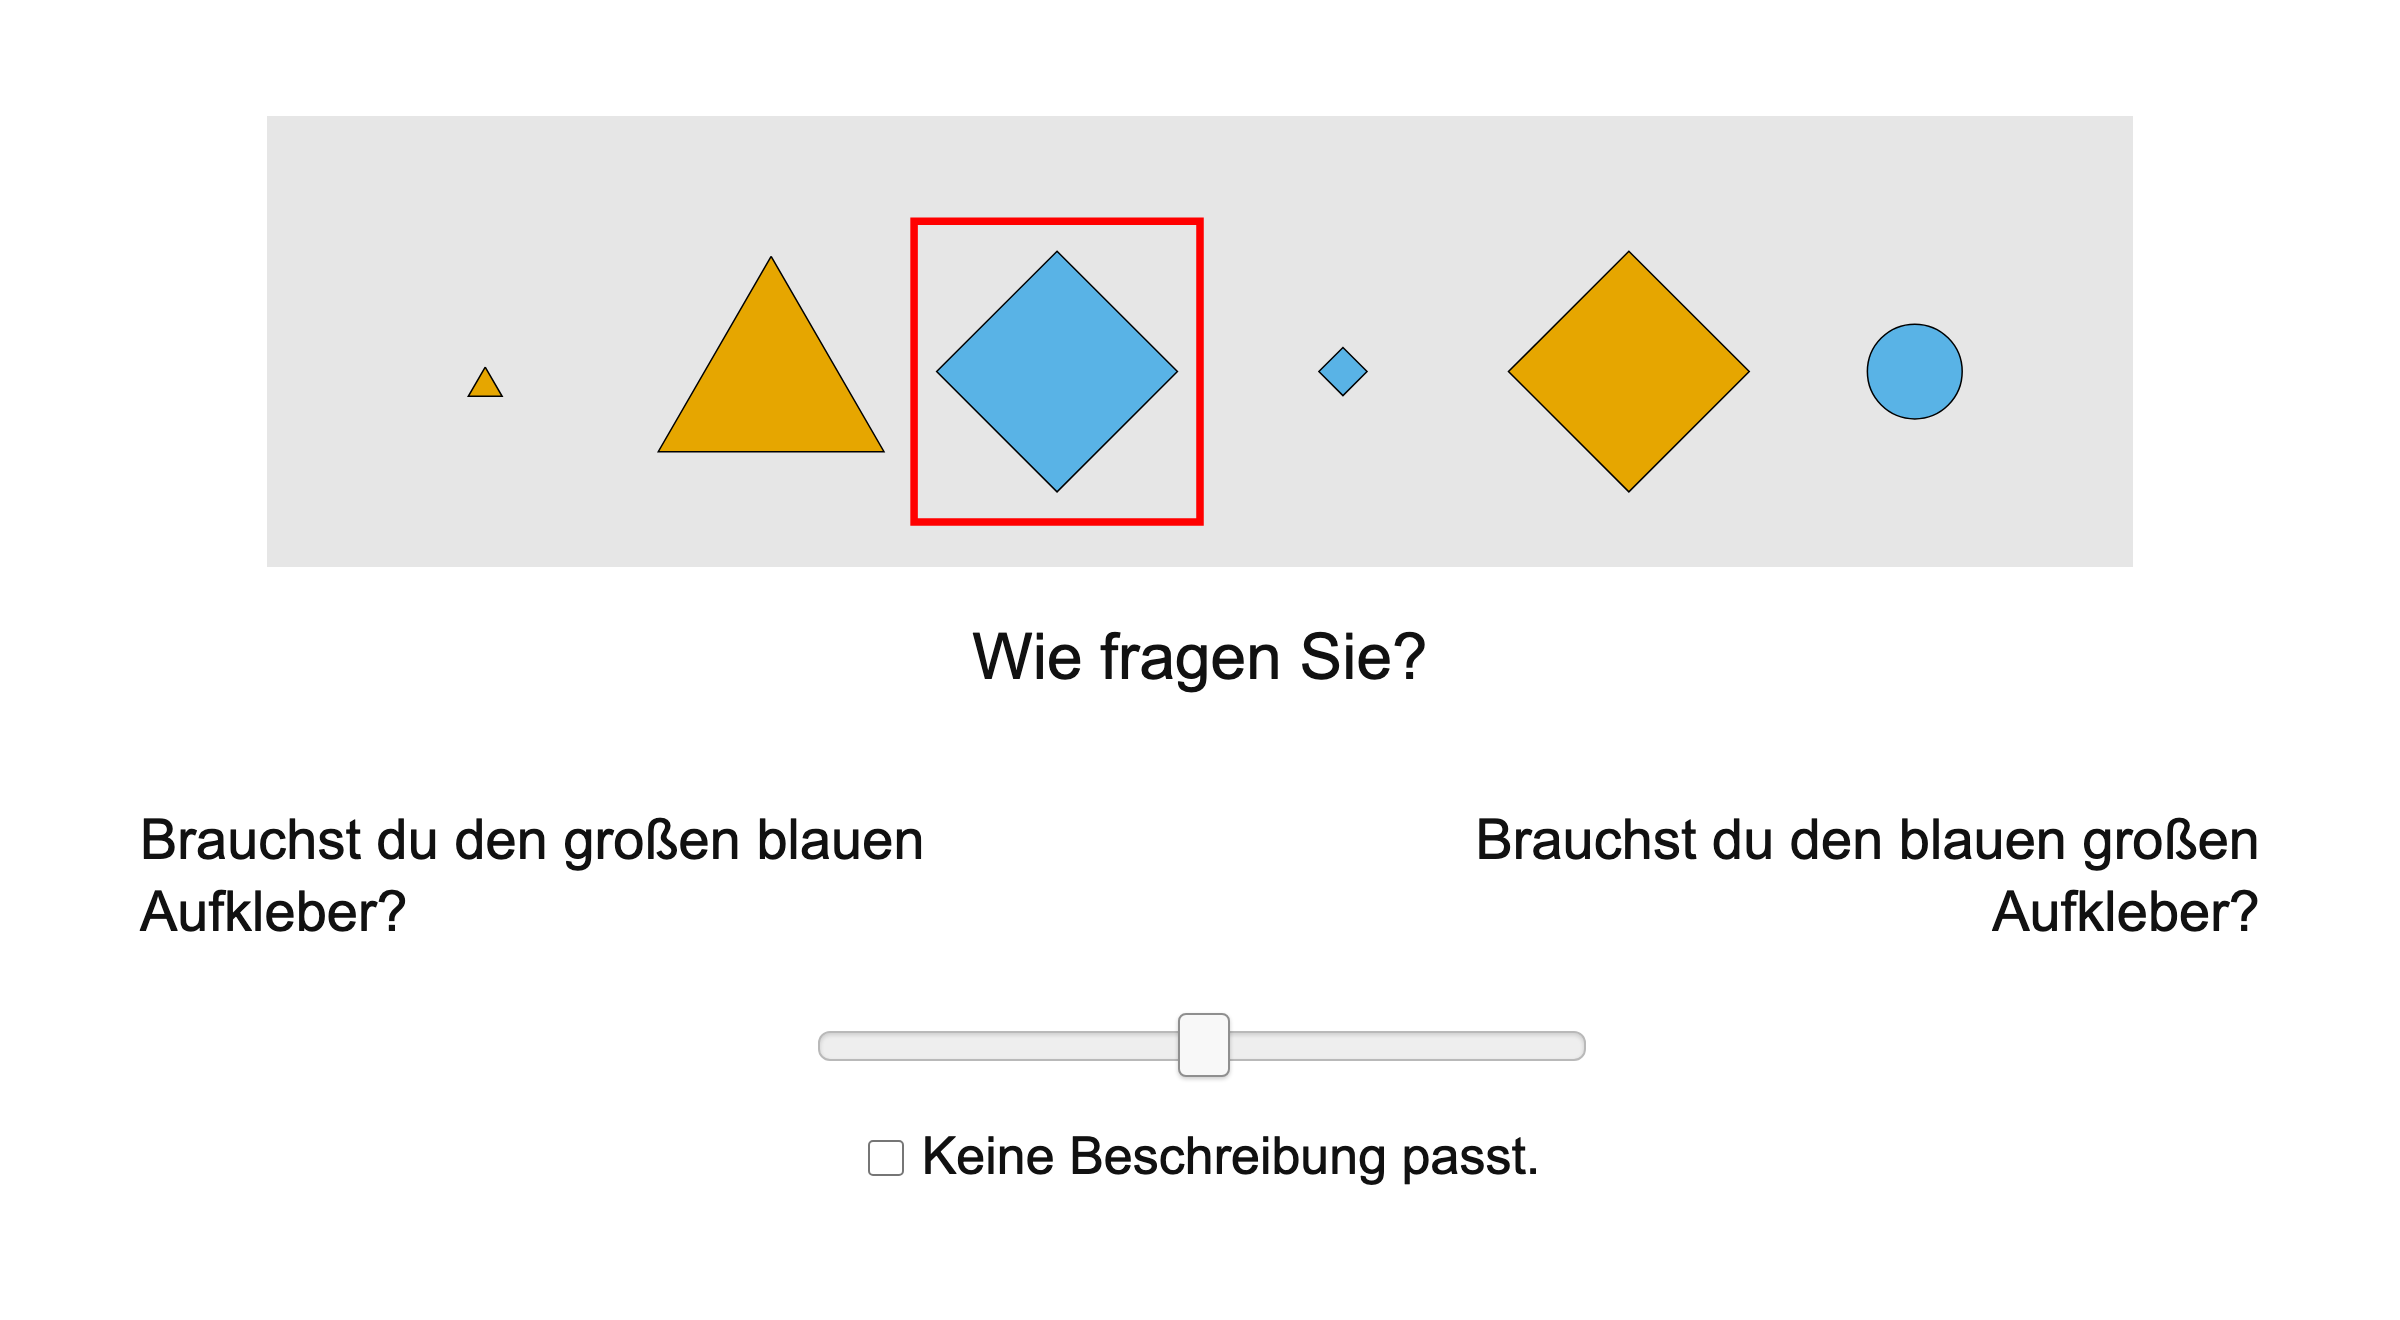
\includegraphics[width=\linewidth]{experiment_trial_snapshot.png}
  \end{minipage}
  \caption{Experimental design and materials.
  Panel A summarises the shared design dimensions and task coverage.
  Panel B reproduces an exact slider-trial screenshot: the framed object is the target, and participants rated the two German adjective orders.}
  \label{fig:design}
\end{figure}

\subsubsection{Materials}

Items were distributed across participants in a Latin-square design, so that scene templates and condition assignments were counterbalanced across lists.
In addition to list counterbalancing, the critical scenes were realised through systematic permutations of colour and form values.
This created variability in the surface displays and preserved the referential structure required by each condition.
These permutations were applied to 27 critical scene templates, each specifying an abstract six-object configuration with a target, competitors, and distractors.
Critical vocabularies were fixed across the study, with six colour terms and six form terms reused throughout the scene set; the modified noun was always \textit{Aufkleber} (`sticker').%
\footnote{The form values were presented with German adjectival forms, such as \emph{runden} for round/circle and \emph{quadratischen} for square, so that form could occupy the same prenominal adjective position as colour and size.}
The computational analysis reconstructed each display deterministically from the raw stimulus record as a $6 \times 3$ matrix, with one row per object and columns for observed size ($s$), colour ($c$), and form ($f$).
The referent was stored at index 0.
Participants saw the corresponding visual arrays; no stochastic feature recoding enters the final analysis.

\subsubsection{Procedure}

All studies were conducted online via Prolific.
Participants in each experiment were instructed to identify the framed target using its perceptual properties.
Spatial descriptions such as \emph{left} or \emph{right} were excluded.
The task was framed as a simple reference game about collectible stickers: participants saw one framed target and gave or evaluated a description for a partner who saw the same stickers in a different order and lacked the target frame.
This made spatial terms uninformative and kept the task focused on adjective descriptions.
Each study began with a consent form and a brief practice block (three training trials with feedback) that familiarised participants with the interface and the referential task.
The main trials were divided into four blocks of approximately equal length, with self-paced breaks between blocks.
Trial order within each block was randomised independently for each participant.
The experiment-specific response formats, trial counts, and response coding are reported below.


\subsection{Study 1a: Slider-Rating Study}
\label{sec:exp:slider}

\subsubsection{Participants}

Participants ($N = 134$ after exclusions; 70 in the \textsc{low} size discriminability group, 64 in the \textsc{high} size discriminability group) were recruited online via Prolific and reported German as their native language.
Exclusion criteria were: more than three missing trial-list entries, completion times more than two standard deviations from the sample mean, more than three failures on control items, or more than three ``none fits'' responses on experimental items.%
\footnote{Control items were filler trials with an unambiguous expected response, included to screen for inattentive or non-referential responding.
The additional ``none fits'' option allowed participants to indicate that neither description identified the target; frequent use of this option on experimental items was treated as evidence of a response strategy outside the intended comparative-judgment task.}
After exclusions, the analysed dataset contained 10{,}606 critical observations.
The size--colour subset reported in the main empirical and model-comparison figures contained 3{,}485 observations; the appendix summarises exclusion details.
Mean completion time was 27.6 minutes.
Participants were compensated via Prolific at a rate above the platform-recommended minimum.

\subsubsection{Procedure}

Study~1a implemented the shared referential design as a comparative judgment task.
On each critical trial, two competing adjective orders appeared on opposite sides of a continuous slider, together with a ``none of the descriptions fits'' option.
Left--right presentation of the two orders was randomised across trials.
Each participant saw one of six lists built from the 27 underlying scenes, yielding 81 critical trials and 99 filler and control trials (180 total).
The filler and control items discouraged fixed response strategies and ensured attention to the referential task.
Responses were reoriented so that larger values favoured the size-first order and rescaled from 0--100 to 0--1.
We then subtracted $0.5$, yielding a centred scale from $-0.5$ to $0.5$ with zero as the neutral point.

\subsubsection{Results}

\Cref{fig:slider-empirical} shows a clear referential-context gradient in size-first ratings.
We analysed the centred ratings with a Bayesian Gaussian hierarchical model containing referential context, size discriminability, and their interaction, together with correlated participant intercepts and participant slopes for referential context.
Planned hypotheses were evaluated through population-level expected ratings; we report posterior medians, $95\%$ credible intervals, and directional posterior probabilities.

Mean centred ratings, indexing preference for size-first orderings, were highest in size-sufficient displays, lower in both-necessary displays, and lowest in colour-sufficient displays.
Mean centred ratings remained above zero in colour-sufficient contexts, yielding no qualitative reversal.
The posterior contrast between size-sufficient and both-necessary displays was $.094$, $95\%$ credible interval $[.061,.127]$, and the contrast between both-necessary and colour-sufficient displays was $.171$, $[.131,.208]$.
The posterior probability of this graded context order was greater than $.999$.
It estimated a colour-sufficient preference of $.054$, $95\%$ credible interval $[.003,.109]$, with posterior probability $.982$ of exceeding the neutral point.

The high-minus-low discriminability contrast was $.042$, $95\%$ credible interval $[-.013,.099]$, in size-sufficient displays, $-.043$, $[-.118,.028]$, in both-necessary displays, and $-.021$, $[-.129,.082]$, in colour-sufficient displays.
The interaction contrast comparing the high-minus-low effect in both-necessary with size-sufficient displays was $-.085$, $95\%$ credible interval $[-.151,-.022]$, with posterior probability $.995$ of being below zero.
The corresponding colour-sufficient versus size-sufficient interaction contrast was $-.063$, $95\%$ credible interval $[-.172,.039]$, with posterior probability $.885$ of being below zero.
The descriptive crossover is therefore concentrated in the difference between size-sufficient and both-necessary contexts, while the colour-sufficient component remains uncertain.
Study~1b provides the direct test of whether this interaction pattern recurs.
The central result is therefore a size-first preference graded by referential usefulness: it was strongest when size alone identified the target, weakest when colour alone did, and remained slightly positive in the colour-sufficient condition.

\begin{figure}[H]
  \centering
  
\includegraphics[width=0.88\textwidth]{slider_empirical.pdf}
  \caption{Slider-rating data.
  Mean centred slider ratings by referential context and size discriminability, with $95\%$ confidence intervals; positive values indicate size-first preference.}
  \label{fig:slider-empirical}
\end{figure}


\subsection{Study 1b: Direct Slider Replication}
\label{sec:exp:slider-replication}

\subsubsection{Participants and preprocessing}

The replication retained 104 of 132 participants after applying the Study~1a exclusions to an independent participant sample.
The cleaned file contains the same 1{,}080 list--item--condition design tuples as Study~1a and 8{,}379 critical observations.
The size--colour subset contained 2{,}786 observations.
The complete exclusion and preprocessing record appears in \Cref{sec:appendix:methods-transparency}.

\subsubsection{Results}

We fitted the same Bayesian Gaussian hierarchical model as in Study~1a to the replication ratings.
Mean centred ratings were $0.272$ in size-sufficient contexts, $0.197$ when both properties were necessary, and $0.054$ in colour-sufficient contexts.
The posterior contrast between size-sufficient and both-necessary displays was $.073$, $95\%$ credible interval $[.029,.115]$, and the contrast between both-necessary and colour-sufficient displays was $.140$, $[.090,.190]$.
The posterior probability of the graded context order was $.999$.
It estimated the colour-sufficient preference at $.057$, $95\%$ credible interval $[.001,.116]$, with posterior probability $.977$ of exceeding neutrality.
Study~1b therefore directly replicates the primary context gradient and supplies convergent evidence for a small positive colour-sufficient preference.
High discriminability was associated with higher ratings in all three contexts, by $.090$, $95\%$ credible interval $[.014,.160]$, in size-sufficient displays, $.076$, $[-.011,.161]$, in both-necessary displays, and $.124$, $[.016,.240]$, in colour-sufficient displays.
The interaction contrast comparing both-necessary with size-sufficient displays was $-.014$, $95\%$ credible interval $[-.097,.071]$, with posterior probability $.623$ of being below zero.
The corresponding colour-sufficient versus size-sufficient interaction contrast was $.034$, $95\%$ credible interval $[-.082,.157]$, with posterior probability $.715$ of exceeding zero.
The Study~1a crossover therefore does not recur.
Study~1b shows a broadly shared high-discriminability shift across contexts.
Size discriminability therefore remains secondary to the replicated context gradient.

\begin{figure}[H]
  \centering
  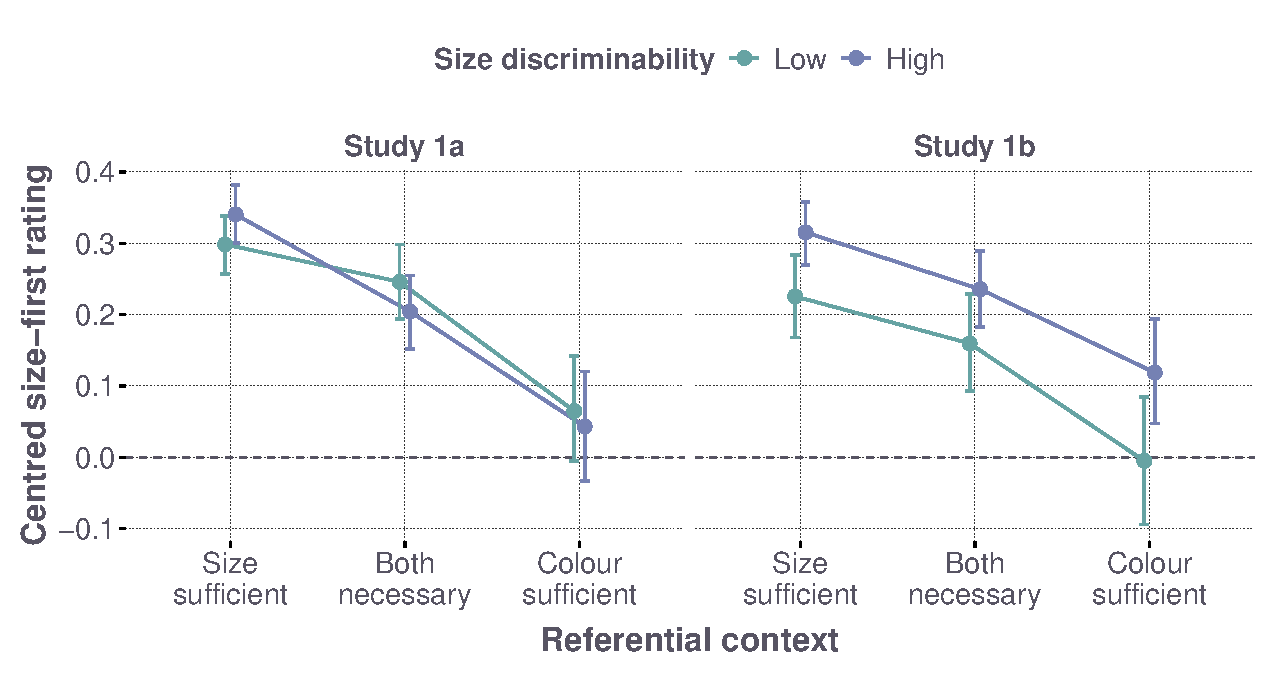
\includegraphics[width=0.88\textwidth]{study1_slider_replication.pdf}
  \caption{Combined Study~1a and Study~1b slider results.
  Mean centred ratings by referential context in each study, with $95\%$ confidence intervals over participant-level means; positive values indicate size-first preference.}
  \label{fig:slider-replication}
\end{figure}


\subsection{Study 2: Production Study}
\label{sec:exp:production}

\subsubsection{Participants}

Participants ($N = 113$ after exclusions; 60 in the \textsc{low} size discriminability group, 53 in the \textsc{high} size discriminability group) were recruited online via Prolific; anyone who had completed either slider study was excluded.
Further exclusion criteria were: completion times more than two standard deviations from the mean, more than 80\% identical responses, or more than 10\% missing or unannotatable responses.
The canonical production table contains 9{,}100 annotated observations across all three adjective-pair families.
The model comparison retains the native fifteen-category response space across size--colour, size--form, and colour--form trials.
Adjective family is a structured dimension of the materials that specifies which two properties support reference; the primary experimental factors remain referential context and size discriminability.
The targeted Bayesian hypothesis tests use the 3{,}034 size--colour trials to align directly with the slider studies, while size--form provides generalisation to a second size-containing family and colour--form provides a control for the full-data model comparison.
Mean completion time was 32.4 minutes.
Compensation followed the same Prolific rate as Study~1a.

\subsubsection{Procedure}

Study~2 used the shared referential design in a production format.
Participants saw the framed target together with the fixed sentence frame \emph{den \_\_\_ Aufkleber} and typed the adjective material needed before the noun \textit{Aufkleber}.
Restricting the response to the adjective slot reduced off-task variability and provided a controlled basis for coding.
The practice materials additionally introduced the relevant colour and form vocabulary before the critical trials began.
Each participant completed 135 main trials: 81 critical trials and 54 filler or control trials from one of six counterbalanced lists.%
\footnote{The number of filler and control trials was reduced in Study~2 to keep the total number of trials manageable because typed production responses were slower and more effortful than slider judgments.}

Responses were coded into 15 utterance categories corresponding to all ordered combinations of \adj{S} (size), \adj{C} (colour), and \adj{F} (form): 3 one-adjective, 6 two-adjective, and 6 three-adjective strings.
Misspellings and transparent lexical alternatives were normalised when their semantic class was unambiguous; spatial descriptions, comparative or ordinal size expressions, and other unclassifiable responses were excluded.
The dependent variable for the Bayesian model comparison is the categorical utterance label $y_i \in \{1, \ldots, 15\}$ for each trial $i$.
For supplementary comparison with the slider studies, we also tracked two derived binary projections: whether an utterance was size-initial and whether it contained more adjective material than the minimally sufficient property set.
These projections combine several underlying choices and are not treated as direct measures of adjective order.
Each projection was analysed with a Bayesian Bernoulli hierarchical model containing referential context, size discriminability, and their interaction, correlated participant intercepts and participant slopes for referential context, and an item intercept.
Trials satisfying the coded outcome were coded as $1$ and all other annotated size--colour trials were coded as $0$.
The planned interaction contrasts were evaluated through posterior-predictive response probabilities for a new participant and item.



\subsubsection{Results}

\Cref{fig:production-distribution} provides an overview of the ordered response distribution for the 3{,}034 size--colour trials, which align directly with the slider studies and the targeted behavioural tests.
The computational analysis below retains all 9{,}100 production trials across size--colour, size--form, and colour--form.
The complete categorical distribution shows that referential context affects which adjectives are selected and how much adjective material is produced.
Both-necessary scenes generally elicit longer descriptions, whereas one-property-sufficient scenes more often elicit a single adjective.
In particular, colour-sufficient size--colour scenes are commonly resolved with colour alone.
On those trials, no size--colour ordering decision is observed.

\paragraph{Selection, adjective set, and length.}
In the size--colour trials, speakers preferentially mentioned properties that distinguished the target in the current scene.
The resulting unordered adjective-set distribution separates one-property responses from responses that contain both referentially relevant properties and from three-adjective descriptions.
Lower size discriminability increased the probability of additional adjective material most clearly when size alone would otherwise have been sufficient.
\Cref{fig:production-recodings}A isolates this pattern through the over-informative-response recoding used in the targeted hypothesis test.
In the supplementary binary projection, over-informative responses were more frequent under low than high size discriminability in size-sufficient displays ($.90$ vs.\ $.63$).
The posterior-predictive low-minus-high difference was $.234$, $95\%$ credible interval $[.151,.318]$, with posterior probability greater than $.999$ of exceeding zero.
The planned interaction compared this difference with the mean low-minus-high difference in the both-necessary and colour-sufficient contexts; it was $.153$, $95\%$ credible interval $[.072,.236]$, with posterior probability greater than $.999$ of exceeding zero.
The visual manipulation therefore bears most clearly on adjective selection and utterance length, with weaker evidence for a stable ordering preference.

\paragraph{Initial adjective and conditional order.}
Initial-adjective probabilities reflect both whether an adjective is selected and where it occurs.
For this reason, size-initiality provides a useful descriptive projection of the complete response space whose probability reflects more choices than the slider outcome.
\Cref{fig:production-recodings}B shows the size-initial recoding used in the targeted hypothesis test.
High discriminability increased size-initial responses in both-necessary displays ($.49$ vs.\ $.65$), with a posterior-predictive difference of $.141$, $95\%$ credible interval $[.036,.242]$, and posterior probability $.997$ of exceeding zero.
The planned interaction compared this difference with the mean high-minus-low difference in the two one-property-sufficient contexts; it was $.169$, $95\%$ credible interval $[.077,.256]$, with posterior probability greater than $.999$ of exceeding zero.
The corresponding difference was $-.021$, $95\%$ credible interval $[-.101,.057]$, in size-sufficient displays and $-.032$, $[-.068,-.006]$, in colour-sufficient displays.
This interaction concerns the joint outcome of selecting size and placing it initially in the completed response.
Conditional on producing both size and colour, size-first descriptions remained more frequent than colour-first descriptions; colour-before-size reversals were comparatively rare.
That conditional subset is selected by the prior decision to mention both properties and is therefore reported separately from adjective selection and length.
The same distinction applies to size--form, colour--form, and three-adjective responses.

\begin{figure}[H]
  \centering
  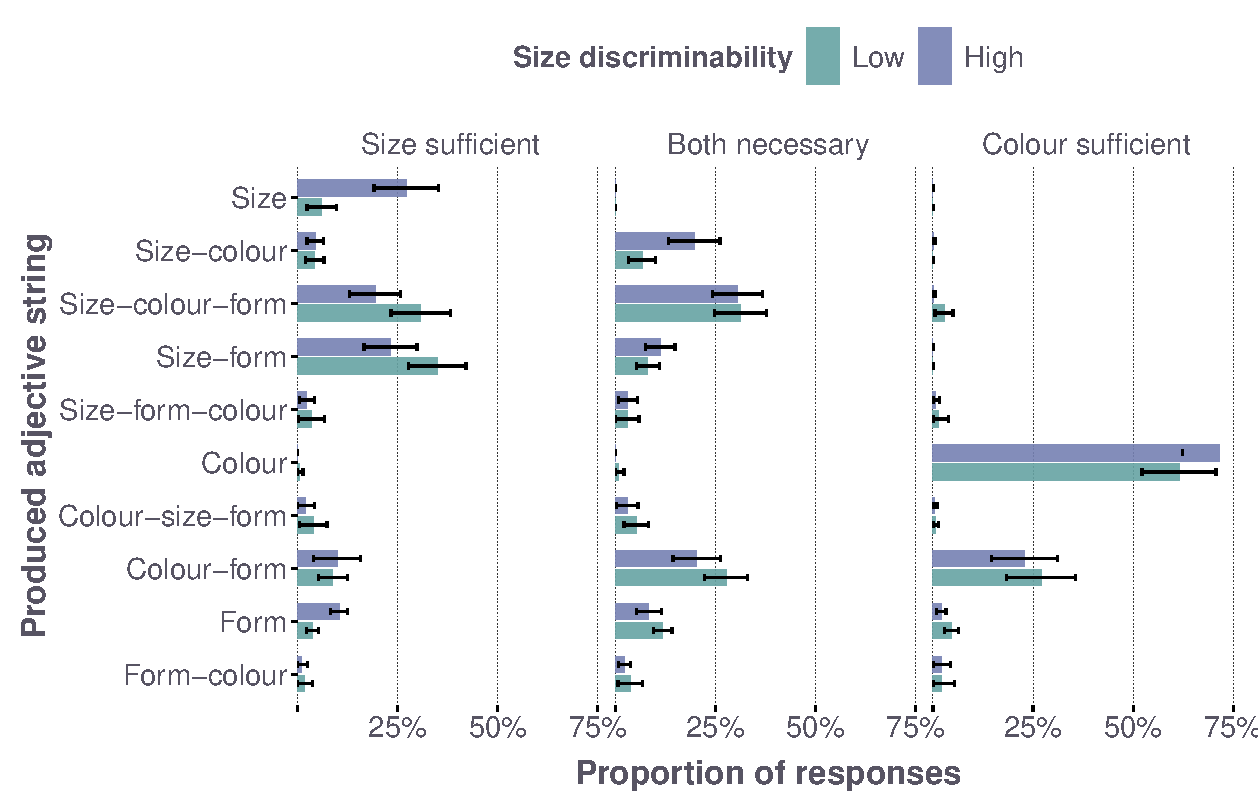
\includegraphics[width=0.95\textwidth]{production_distribution.pdf}
  \caption{Ordered response distribution across the 3{,}034 size--colour production trials.
  Bars show mean participant-level proportions by referential context and size discriminability, with $95\%$ confidence intervals.
  Adjective labels preserve surface order; the figure shows responses reaching at least $2\%$ in one condition.}
  \label{fig:production-distribution}
\end{figure}

\begin{figure}[H]
  \centering
  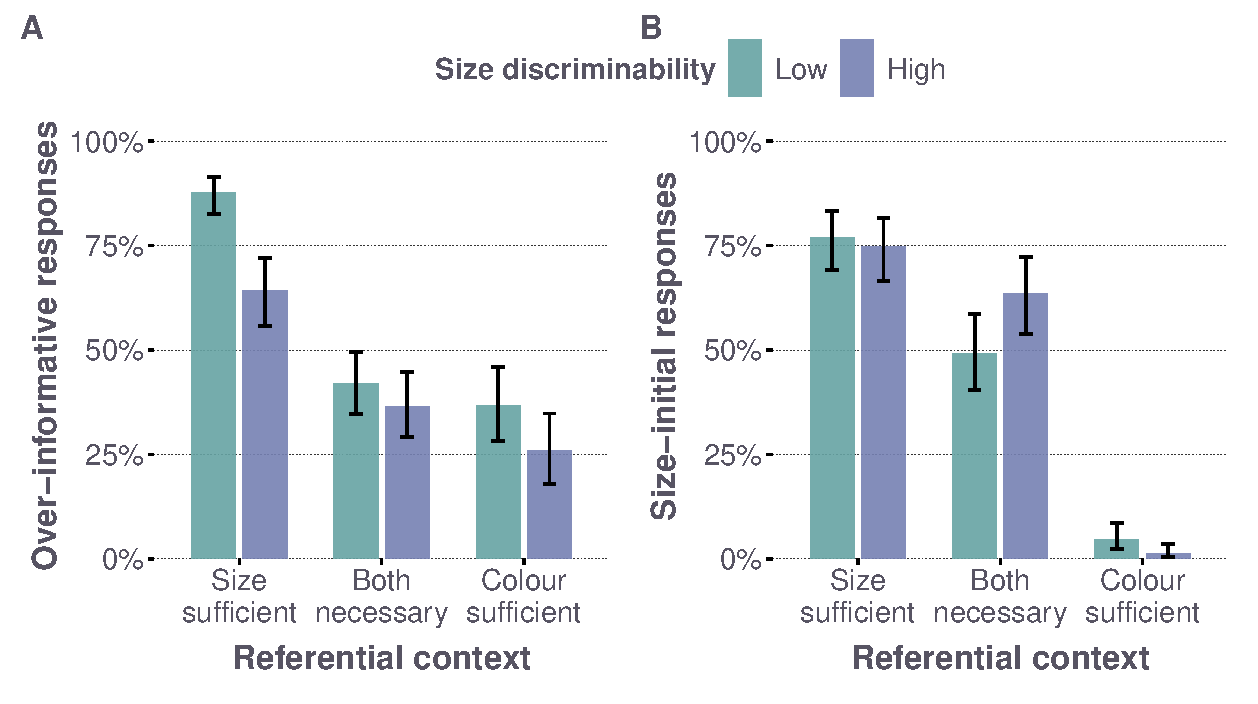
\includegraphics[width=0.95\textwidth]{production_hypothesis_recodings.pdf}
  \caption{Hypothesis-linked recodings of the size--colour production responses.
  Panel A codes redundant adjective use as over-informative: a multi-adjective response in a one-property-sufficient context or a three-adjective response when both properties are necessary.
  Panel B codes whether the response begins with size.
  Bars show Bayesian posterior medians and error bars show $95\%$ credible intervals.
  Size-initiality combines adjective selection and order.}
  \label{fig:production-recodings}
\end{figure}

\subsection{Discussion}

The two response formats expose different stages at which communicative efficiency can affect adjective ordering.
The slider studies establish a replicated context gradient in explicit comparisons between two completed size--colour orders.
Ratings are highest when size identifies the target, lowest when colour does, and retain a small positive size-first estimate in the colour-sufficient condition.
Direct production allows the same referential context to affect earlier choices about adjective selection and utterance length.
When one property identifies the target, speakers frequently produce a single adjective and stop before an order among multiple adjectives becomes observable.
The context manipulation can therefore shift direct judgements between completed orders and also determine whether production reaches an ordering choice at all.

The interaction between size discriminability and referential context differs across tasks and production outcomes.
In Study~1a, the interaction is concentrated in the contrast between size-sufficient and both-necessary displays, with weaker evidence for the colour-sufficient component.
Study~1b shows a broadly shared high-discriminability shift across contexts, and both interaction contrasts remain uncertain.
The slider studies therefore replicate the referential-context gradient while providing limited evidence for a stable discriminability-by-context interaction in explicit order judgements.
Study~2 shows stronger outcome-specific interactions within direct production.
Lower size discriminability increases additional adjective material most clearly in size-sufficient scenes, whereas higher size discriminability increases size-initial responses most clearly when both size and colour are necessary.
These production interactions locate the effect in adjective selection, utterance length, and initial position before order is examined conditional on a fixed adjective set.
Their magnitudes are expressed on response-probability scales, while the slider interactions are expressed on the centred-rating scale.
The reported production hypothesis tests and \Cref{fig:production-distribution,fig:production-recodings} are restricted to the size--colour trials, preserving direct comparability with the slider studies.
A descriptive check of the complete production data shows that the between-participant manipulation also changes responses in the colour--form family, where colour and form define the referential contrast.
In form-sufficient displays, for example, form-initial responses are more frequent in the high- than in the low-discriminability group ($.77$ vs.\ $.71$).
This cross-family pattern is consistent with a broader amplification of scene-specific sufficiency and indicates that the manipulation may capture task-wide differences between participant groups alongside changes in the perceptual reliability of size.
The behavioural manipulation therefore cannot by itself identify the contribution of sequential context updating within hierarchical semantic composition.
This limitation motivates the controlled simulation, which varies the semantic consequences of sequential context updating directly and asks when they are sufficient to generate an ordering asymmetry.

Production also reveals substantial use of maximal three-adjective utterances and pronounced participant heterogeneity in how often these longer utterances occur.
Three-adjective responses are theoretically informative because speakers continue beyond the material required for unique reference and traverse multiple adjective positions before completing the utterance.
Participant heterogeneity further raises the possibility that the pressures governing adjective selection, length, and successive adjective choice differ across speakers.
These qualitative patterns motivate a model of the complete fifteen-category response distribution with participant-level variation.
An isolated size-first/colour-first contrast captures only the responses in which both adjectives have already been selected.


% =============================================================================
\section{Formal Modelling Framework}
\label{sec:model}
% =============================================================================

The formal framework of the current paper builds on the central intuition of the Rational Speech Act (RSA) model: rational communication links comprehension and production, such that a listener interprets an utterance to infer the speaker's intended referent and a pragmatic speaker assigns greater probability to utterances that guide the listener successfully to the target \citep{frank2012predicting}.\
In the vanilla RSA model, the speaker evaluates a fixed set of completed utterances according to their communicative efficiency.\
The present model extends the vanilla RSA model in three respects.\
First, it expands the response space to all fifteen ordered one-, two-, and three-adjective utterances available in the experiment, bringing adjective selection, utterance length, and ordering into a single production distribution.\
This extends the two fixed size--colour orders modelled by \citet{schlotterbeck2023incremental} to the richer structure of adjective use observed in direct production.\
Second, it allows recursive updating of the listener state as adjectives modification computes within hierarchical semantic composition.\
Third, it extends the speaker to incremental production by allowing adjective choices to be evaluated successively along the surface linear sequence.\

The last two extensions represent the two directions through which communicative efficiency may shape adjective ordering.\
Along the surface linear sequence, each adjective changes the alternatives available at the next position.\
The production architecture determines how strongly these successive evaluations contribute to the probability of the completed utterance, ranging from global evaluation through plan-guided production to fully incremental adjective choice.\
Within hierarchical semantic composition, adjectival modification proceeds from the noun outwards.\
Sequential context updating allows a noun-adjacent adjective to restrict the comparison class relative to which gradable size is interpreted.\

The section develops these components in the following steps.\
We first define the utterance space, visual state space, and literal listener that are shared by all models.\
We then formalise global, plan-guided, and fully incremental production as alternative ways of assigning probabilities to completed utterances.\
Finally, we define how size is interpreted under context-fixed semantics and sequential context updating within hierarchical semantic composition.\
Additionally, all models include shared components that account for task-specific production patterns in adjective selection and utterance length, together with stable order expectations and perceptual salience.\
Their complete parameterisation and supporting robustness analyses are documented in the Appendix.\

\subsection{Utterance Space, State Space and the Literal Listener}
\label{sec:model:response-space}

The model assigns probabilities to all fifteen ordered strings formed from size, colour, and form: three one-adjective utterances, six two-adjective utterances, and six three-adjective utterances.
This response space allows the model to predict which properties speakers mention, how many adjectives they produce, and how jointly selected adjectives are ordered.
All models use the observed six-object display and a Rational Speech Act speaker who favours utterances that guide a listener to the target \citep{frank2012predicting,goodman2016pragmatic,degen2023rational}.
Size has a graded meaning defined relative to a comparison class \citep{schmidt2009how,franke2019subjectivity}.
Colour and form provide additional visual information about the target.

Let $u_{\leq t}=w_1\ldots w_t$ be a surface prefix and $P_0(o)$ the prior probability of object $o$ in the display.
Under context-fixed semantics, the literal listener after this prefix is
\begin{equation}
  Q_t(o\mid u_{\leq t})
  \propto
  P_0(o)\prod_{j=1}^{t}
  \llbracket w_j\rrbracket_{\mathrm{fix}}(o).
  \label{eq:prefix-listener}
\end{equation}
The listener combines the meanings made available by the surface prefix and assigns probability to every object that remains compatible with them.
This listener provides the target-directed value used by all three production accounts.

\subsection{Successive Adjective Choice and Plan-Guided Production}
\label{sec:model:architectures}

At position $t$, the utility of candidate adjective $a$ for participant $i$ and target $o^*$ is
\begin{equation}
  r_{it}(a;u_{<t},o^*)
  = \alpha_i\log Q_t(o^*\mid u_{<t}+a)
  + \lambda_{\mathrm{salience}}z_a,
  \label{eq:prefix-raw-utility}
\end{equation}
where $\alpha_i$ controls sensitivity to listener success and $z_a$ represents the visual salience of the candidate property.
For a completed utterance $u$, the model records both the accumulated utility of its selected adjectives and the competition they faced at successive positions:
\begin{align}
  R_i(u,o^*)
  &=\sum_t r_{it}(w_t;u_{<t},o^*),\\
  N_i(u,o^*)
  &=\sum_t\log\!\sum_{a\in\mathcal A(u_{<t})}
    \exp r_{it}(a;u_{<t},o^*),
  \label{eq:path-components}
\end{align}
where $\mathcal A(u_{<t})$ contains the adjective types still available after the current prefix.
The term $R_i$ scores the selected path through the utterance.
The term $N_i$ accumulates the local normalisers associated with the alternatives available along that path.
All three accounts therefore use the target-directed values of intermediate prefixes contained in $R_i$.

The probability of a completed utterance is
\begin{equation}
  S_{\kappa,i}(u\mid o^*,X)
  \propto
  \exp\!\left\{
    R_i(u,o^*)
    -\kappa N_i(u,o^*)
    +\beta_i\Omega(u)
    +T(u,X)
  \right\},
  \label{eq:plan-guided-speaker}
\end{equation}
where $\Omega(u)$ is a German language model's relative score for alternative orders of the same adjectives and $\beta_i$ allows its influence to vary across participants.
The task link $T(u,X)$ captures adjective selection and utterance length through the observed effects of adjective sufficiency, form use, size reliability, and length.
These terms are shared across the three production accounts.

At common values of the shared parameters, the same model can be written as a geometric interpolation between the global and fully incremental endpoints:
\begin{equation}
  S_{\kappa,i}(u\mid o^*,X)
  \propto
  S_{\mathrm{G},i}(u\mid o^*,X)^{1-\kappa}
  S_{\mathrm{I},i}(u\mid o^*,X)^{\kappa},
  \label{eq:plan-guided-interpolation}
\end{equation}
where $S_{\mathrm{G},i}$ and $S_{\mathrm{I},i}$ are the endpoint distributions evaluated with the same listener, stable-order component, task link, and participant parameters.
The proportionality in \Cref{eq:plan-guided-interpolation} renormalises the interpolated scores over the fifteen completed utterances.

The parameter $\kappa$ determines how strongly competition at successive adjective positions contributes to the completed-utterance probability.
With $\kappa=0$, the local normalisers drop out and the \emph{global} speaker normalises over the fifteen completed paths.
With $\kappa=1$, the \emph{fully incremental} speaker retains the complete contribution of locally normalised adjective choices.
An interior value defines the \emph{plan-guided} speaker: an advance utterance plan constrains the completed response, and competition among locally available adjectives continues to shape its surface realisation.
Stopping enters through $T(u,X)$ at the completed-response level.
Accordingly, $\kappa$ measures the contribution of successive adjective choice.
Online stopping and the time course of planning remain outside its interpretation.

\subsection{Sequential Context Updating in Hierarchical Composition}
\label{sec:model:semantic-comparison}

The semantic comparison concerns the inner-to-outer direction of hierarchical composition.
Let $c_1,\ldots,c_T$ denote the modifiers in a completed utterance ordered from the noun outwards, so that $c_1=w_T$ for prenominal modification.
Starting from $H_0=P_0$, composition successively restricts the listener state:
\begin{equation}
  H_j(o)
  \propto
  H_{j-1}(o)\,
  \llbracket c_j\rrbracket_{\rho_j}(o),
  \qquad j=1,\ldots,T.
  \label{eq:hierarchical-composition}
\end{equation}
For \emph{big blue sticker}, this path incorporates \emph{blue} before the gradable meaning of \emph{big} applies.

The semantic regime determines the comparison class used for size:
\begin{equation}
  \llbracket \adj{S}\rrbracket_{\rho_j}(o)
  =
  \begin{cases}
    \llbracket \adj{S}\rrbracket_{\theta_{\delta}(\mathcal C)}(o),
      & \text{context-fixed},\\
    \llbracket \adj{S}\rrbracket_{\theta_{\delta}(H_{j-1})}(o),
      & \text{sequential context updating},
  \end{cases}
  \label{eq:hierarchical-size-regimes}
\end{equation}
where $\theta_{\delta}$ derives a graded size threshold from a comparison class and $\mathcal C$ is the original scene.
Under context-fixed semantics, this threshold remains anchored to the original scene.
Under sequential context updating, the threshold is recomputed from the listener state left by the hierarchically prior modifier.
The surface-prefix listener in \Cref{eq:prefix-listener} follows the produced words from left to right.
The hierarchical listener $H_j$ follows semantic composition from the noun outwards.
This comparison asks whether recomputing the size comparison class adds predictive accuracy in the observed production data.
A separate simulation asks when the same operation is sufficient to create an order asymmetry across a broader range of contexts.
The threshold construction and further semantic details appear in \Cref{sec:appendix:model-specification,sec:appendix:semantic-details}.

% =============================================================================
\section{Model Comparison and Predictive Evidence}
\label{sec:modelcomparison}
\label{sec:model:extended}
% =============================================================================

Section~4 formalised how hierarchical semantic composition and successive adjective choice redistribute probability across the same fifteen completed utterances as a function of communicative efficiency.
Within this account, production architecture and semantic regime define two factors in a $3\times2$ design: the production factor ranges from 1. global through 2. plan-guided to 3. fully incremental production, and the semantic factor determines whether the comparison class for size is 1. updated during hierarchical composition or 2. held constant across one given visual szene.
This factorial structure makes the two proposed directions of communicative efficiency directly comparable.
Their contribution to the observed production distribution must now be established through predictive evidence.

In this section, the analysis proceeds from controlled model comparison to model adequacy and interpretation.
The inference setup first separates the two theoretical factors from the shared response space, participant structure, and task-specific components for adjective selection and utterance length, and then specifies the Bayesian inference and predictive-comparison procedures.
Matched predictive contrasts then use approximate leave-one-out expected log predictive density (ELPD) to compare the six cells of the factorial design while holding these shared components constant.
ELPD measures how much probability a model assigns to responses when each response is treated in turn as held out, with higher values indicating better expected prediction of unseen responses.
These contrasts determine whether the completed-utterance distribution favours global, plan-guided, or fully incremental pragmatic production and whether sequential context updating adds predictive accuracy in the present materials.
Posterior predictive checks next compare the posterior predictions of the best-fitted model with the observed distribution, testing whether the selected computational account recovers the broader structure of adjective use established in Study~2.
Dedicated localisation analyses then identify the completed responses for which the best-fitted plan-guided model makes qualitatively different predictions from the global and fully incremental endpoints.
Finally, participant-level random-effects analyses assess how the fitted contribution of successive adjective choice varies across speakers and whether modelling this heterogeneity improves prediction.


\subsection{Inference Setup}
\label{sec:model:development}
\label{sec:model:inference}

We fit each model to the same 9{,}100 production trials from 113 participants using Bayesian inference in NumPyro \citep{phan2019composable}.
Each likelihood evaluation scores all fifteen completed utterances and performs the required semantic composition and prefix-level normalisation.
To make this exact calculation feasible, we precomputed trial-independent utterance and prefix structures, vectorised and compiled the listener and speaker computations in JAX, and ran four NUTS chains on a GPU.
Figure~\ref{fig:production-inference-plate} separates fixed theoretical choices, estimated parameters, participant variation, and observed responses.
The fixed variables $A$ and $S$ index production architecture and semantic regime.
For participant $i$ on trial $t$, the model maps the display and target $X_{it}$ and the stable-order score $\Omega(u)$ to a probability $\pi_{it}(u)$ over the fifteen possible utterances, from which the observed response $y_{it}$ is drawn.
The vector $\boldsymbol\lambda$ collects the shared task-link coefficients for adjective selection and utterance length.
The participant parameters $\alpha_i$, $\kappa_i$, and $\beta_i$ govern pragmatic optimality, successive adjective choice, and stable order expectations.

\begin{figure}[ht]
  \centering
  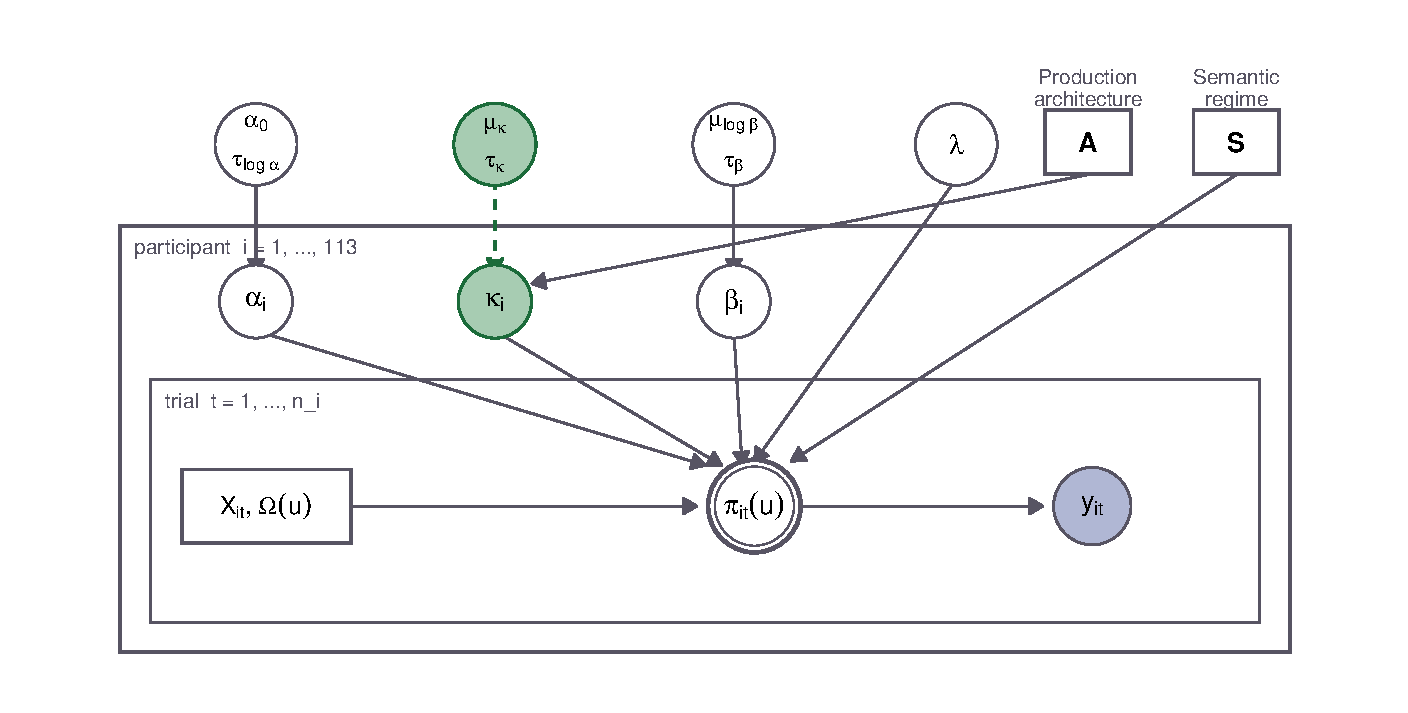
\includegraphics[width=0.97\textwidth]{production_inference_plate.pdf}
  \caption{Formal plate for the final joint hierarchical model and the restrictions used in the matched comparisons.
  Solid circles represent estimated quantities, squares represent fixed model or trial inputs, the double circle represents the deterministic utterance distribution, and the shaded circle represents the observed response.
  The dashed $\kappa$ hierarchy is activated only in the final plan-guided refinement.}
  \label{fig:production-inference-plate}
\end{figure}

Higher $\alpha_i$ increases sensitivity to listener success and concentrates probability on higher-utility responses.
The parameter $\kappa_i$ controls how strongly competition among the adjectives available after an emerging prefix contributes to a completed utterance.
Its endpoints are global production at $\kappa=0$ and fully incremental production at $\kappa=1$.
Higher $\beta_i$ increases the influence of the stable-order score $\Omega(u)$.
The task link includes support for a sufficient one-adjective response, task-conditioned form use, visual reliability, and a shared cost for three-adjective utterances.
The probability of a three-adjective utterance therefore reflects its accumulated referential value and salience, the shared three-adjective cost, and the participant's values of $\alpha_i$, $\kappa_i$, and $\beta_i$.
These quantities identify how the fitted model distributes maximal utterances while remaining agnostic about the cognitive source of redundant production.

The matched $3\times2$ comparison provides two architecture-level tests.
For production, $A$ selects global, plan-guided, or fully incremental production by fixing $\kappa=0$, estimating one shared $\kappa$, or fixing $\kappa=1$.
The plan-guided-minus-endpoints contrast tests whether allowing an intermediate contribution from successive adjective choices improves prediction.
For hierarchical semantic composition, $S$ selects context-fixed semantics or sequential context updating.
The updating-minus-fixed contrast tests whether recomputing the interpretation of size after the noun-adjacent adjective improves prediction.
All six models share the same response space, task link, semantic parameters, and participant hierarchies for $\alpha_i$ and $\beta_i$.
These controls isolate the predictive contribution of each proposed direction of communicative efficiency.

The final refinement is confined to plan-guided production.
It replaces the shared $\kappa$ with a population distribution over participant-specific successive-choice weights $\kappa_i$ and retains the existing hierarchies for $\alpha_i$ and $\beta_i$.
Its predictive comparison tests whether participant variation in successive adjective choice is required.
The population location $\mu_{\kappa}$ and scale $\tau_{\kappa}$ then describe where participants lie between the global and fully incremental endpoints and how widely they vary.
Section~5.2 reports the matched architecture tests, Section~5.3 evaluates the best-fitted refinement and its absolute adequacy, and Section~5.4 localises its gains across utterances and participants.

Approximate leave-one-out prediction compares out-of-sample accuracy for the complete fifteen-response distribution \citep{vehtari2017practical}.
The pointwise score vectors use the same trial ordering and response support.
Because observations are repeated within participants, paired score contributions are first summed within participant.
A participant-level Bayesian bootstrap then assigns Dirichlet weights to the 113 participant contributions over 200{,}000 draws.
Reported uncertainty comprises 95\% credible intervals, posterior probabilities for directional contrasts, and posterior probabilities that semantic effects fall within the predefined $\pm4$-ELPD region of practical equivalence.
The predictive target is an additional completed response from a sampled participant, with that participant's remaining trials available to estimate their participant-specific parameters.
Online planning time remains outside this target.

\subsection{Model-Comparison Results}
\label{sec:architecture-comparison}

The matched comparisons quantify the predictive contribution of each proposed direction of communicative efficiency to completed utterances.

\paragraph{Production architecture.}
Plan-guided production exceeded the average of the global and fully incremental endpoints by $326.280$ ELPD, with a 95\% credible interval of $[241.632,417.363]$ and posterior probability above zero greater than $.999$.
Its marginal predictive accuracy was the highest of the three architectures in $.991$ of the Bayesian-bootstrap draws.
The endpoint contrast remained uncertain: fully incremental minus global production was $-192.079$ ELPD, with a 95\% credible interval of $[-573.371,84.802]$ and posterior probability above zero of $.106$.
Within the matched plan-guided model, the shared successive-choice weight was
\begin{equation}
  \kappa=.447,
  \qquad 95\%~\text{credible interval}=[.404,.490].
  \label{eq:kappa-result}
\end{equation}
The matched comparison supports completed utterance probabilities shaped jointly by the advance utterance plan and competition among successive adjective choices.

\paragraph{Hierarchical semantic composition.}
Sequential context updating minus context-fixed semantics averaged $-.229$ ELPD across the three production architectures, with a 95\% credible interval of $[-1.271,.808]$.
Its posterior probability of falling within the predefined $\pm4$-ELPD region was greater than $.999$.
The architecture-specific effects were likewise small: $-1.121$ ELPD for global production, $.149$ for plan-guided production, and $.285$ for fully incremental production.
The posterior probability that all three effects fell within a four-ELPD range was $.993$.
Under the production constants and actual size--colour displays, recomputing the size threshold changed the target's graded size value and the literal listener's target probability by less than $.001$ on average.
The fitted materials therefore place the model in a regime where sequential context updating has extremely small semantic consequences.
The simulation in \Cref{sec:simulation} evaluates the same operation under conditions in which its semantic consequences are larger.

\begin{figure}[H]
  \centering
  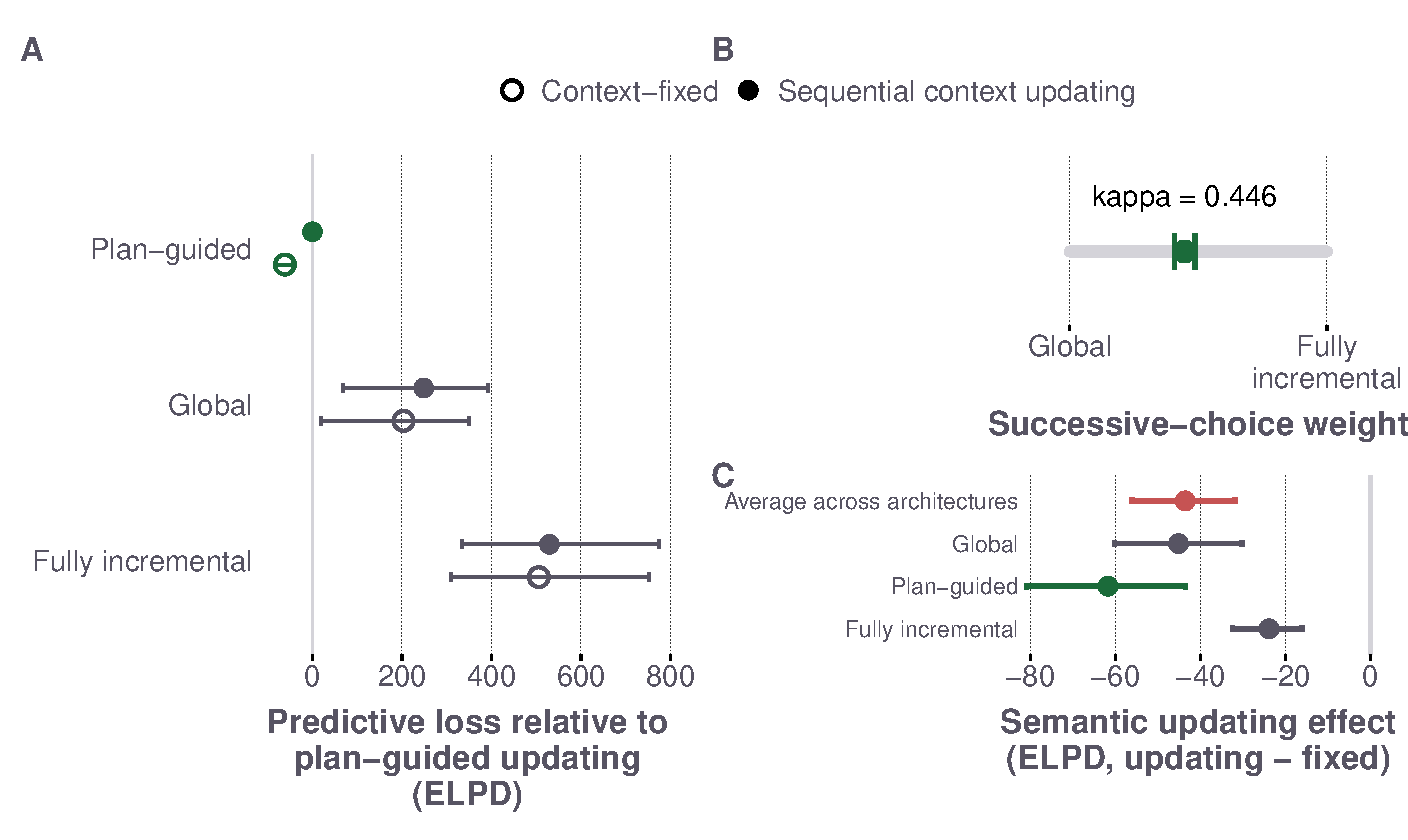
\includegraphics[width=0.95\textwidth]{production_architecture_comparison.pdf}
  \caption{Matched comparisons of production architecture and sequential context updating.
  Panel A reports predictive loss for all six matched models relative to the plan-guided model with sequential context updating; lower values indicate better leave-one-out prediction.
  Panel B places the shared successive-choice weight $\kappa$ between the global and fully incremental endpoints.
  Panel C shows updating-minus-fixed ELPD for each production architecture and their average.
  Intervals are 95\% credible intervals from the participant-level Bayesian bootstrap; the solid vertical line in Panel C marks zero, and the dashed lines mark the predefined $\pm4$-ELPD practical-equivalence boundaries.}
  \label{fig:production-architecture-results}
\end{figure}

\subsection{The Best-Fitted Plan-Guided Model}
\label{sec:architecture-ppc}

The matched comparison identifies the production-architecture advantage with equal participant structure across models.
The final refinement tests whether the contribution of successive adjective choices varies across participants within the plan-guided architecture.
Adding a participant hierarchy for $\kappa_i$ gained $351.425$ ELPD under context-fixed semantics, with a 95\% credible interval of $[239.353,503.120]$, and $352.150$ ELPD under sequential context updating, with a 95\% credible interval of $[240.022,504.081]$.
Both posterior probabilities above zero were greater than $.999$.
The sequentially updating model had the highest numerical ELPD.
The context-fixed version was lower by only $.875$ ELPD, with a 95\% credible interval of $[-.605,2.357]$ and posterior probability of practical equivalence of $.9999$.
Subsequent diagnostics use the sequentially updating model as the best-fitted representative and retain the semantic equivalence conclusion from the matched comparison.

The population location of its participant-specific successive-choice weights was intermediate between the global and fully incremental endpoints, $\mu_{\kappa}=.491$, with a 95\% credible interval of $[.337,.643]$.
The participant distribution was broad, with an estimated logit-scale standard deviation of $2.822$, 95\% credible interval $[2.353,3.329]$.
The model had an absolute ELPD of $-13{,}189.217$, zero divergences, maximum $\widehat R=1.0064$, no observation with Pareto $k>.7$, and minimum BFMI of $.707$.

\Cref{fig:production-architecture-ppc} evaluates its adequacy for the complete observed distribution.
Panel A compares frequent completed utterances in the size--colour trials, where the central ordering contrast arises.
Panel B extends the check to all fifteen completed utterances across the three adjective families, referential contexts, and size-discriminability conditions.
Across these 270 cells, the posterior predictions correlated with the observed proportions at $r=.911$ and $R^2=.830$ ($p<.001$).
The $p$-value is descriptive because cells from the same condition form a compositional distribution and are therefore dependent.
Panel C focuses on size-initial responses and redundant adjective use across referential contexts.
The model captures the broad shifts between one- and multi-adjective utterances across conditions, with visible discrepancies remaining in several cells.

\begin{figure}[H]
  \centering
  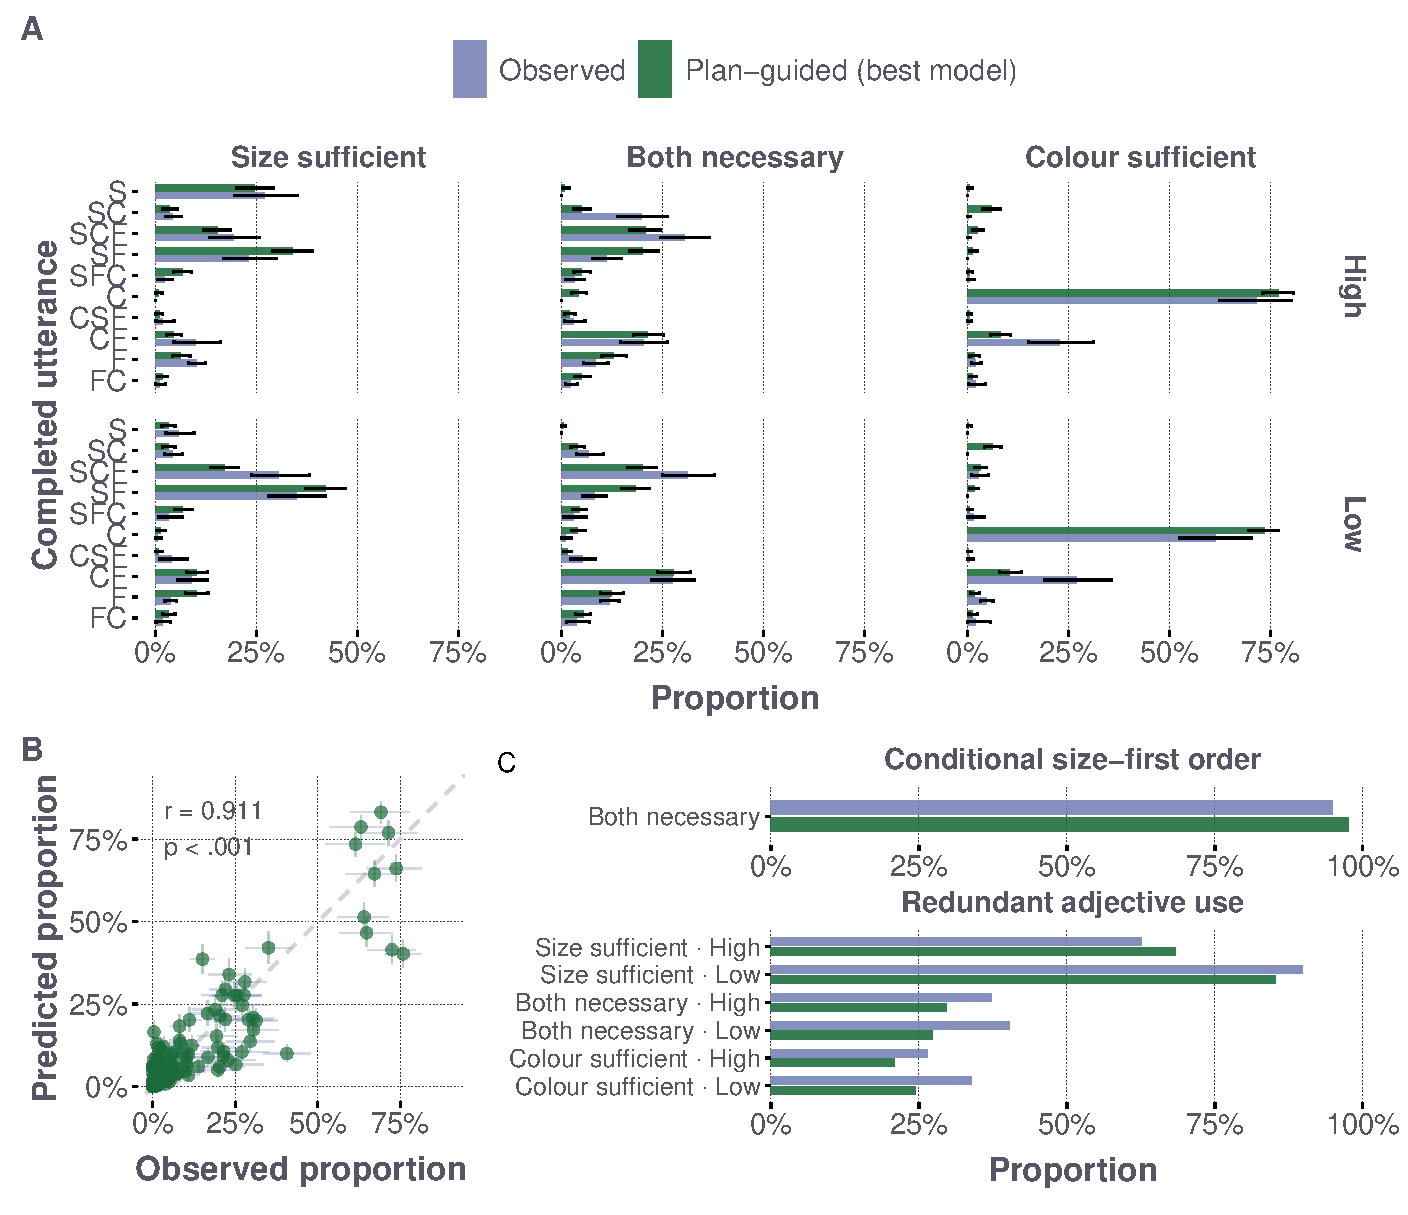
\includegraphics[width=0.95\textwidth]{production_architecture_ppc.pdf}
  \caption{Posterior-predictive adequacy of the best-fitted plan-guided model.
  Panel A shows observed and posterior-predicted proportions with their respective uncertainty intervals for frequent size--colour utterances.
  Panel B compares all 270 cells; horizontal intervals show participant-bootstrap uncertainty in the observations, vertical intervals show 95\% posterior-predictive uncertainty, and the dashed line marks equality.
  Panel C compares observed and posterior-predicted size-initial responses and redundant adjective use, with referential context on the vertical axis and size discriminability in facet rows.
  Intervals in Panel C show participant-bootstrap 95\% intervals for the observed proportions and 95\% posterior-predictive intervals for the model predictions.}
  \label{fig:production-architecture-ppc}
\end{figure}

\subsection{Mechanism and Participant Variation}
\label{sec:architecture-residuals}
\label{sec:participant-variation}

\paragraph{Architecture-level response patterns.}
Qualitative diagnostics localise the distributional patterns that distinguish plan-guided production from its matched endpoints.
\Cref{fig:production-architecture-residuals} shows initial-adjective cells in which the largest difference among architecture predictions is at least 6.7 percentage points and traces these differences into completed utterances.
The largest separations occur in form-involving trials, where colour and form compete for the initial position.
Colour-initial responses contribute $289.682$ of the matched plan-guided model's $326.280$-ELPD advantage over the average endpoint, or $88.8\%$ of the summed pointwise contrast.
Across the displayed cells, plan-guided production often lies between the global and fully incremental endpoints.

Successive normalisation produces this pattern in the model.
The global speaker evaluates the completed utterance distribution.
The fully incremental speaker also normalizes among the adjectives available after each emerging prefix.
Different opening adjectives create different sets of plausible continuations, so competition at later positions redistributes probability among the completed paths that share each initial adjective.
This redistribution has larger consequences when several properties remain viable, especially when colour and form compete in form-involving displays.
The plan-guided speaker gives this prefix-specific competition a participant-specific weight, preserving constraints from the completed utterance and allowing continuation alternatives to reshape its surface realisation to different degrees across participants.

\begin{figure}[H]
  \centering
  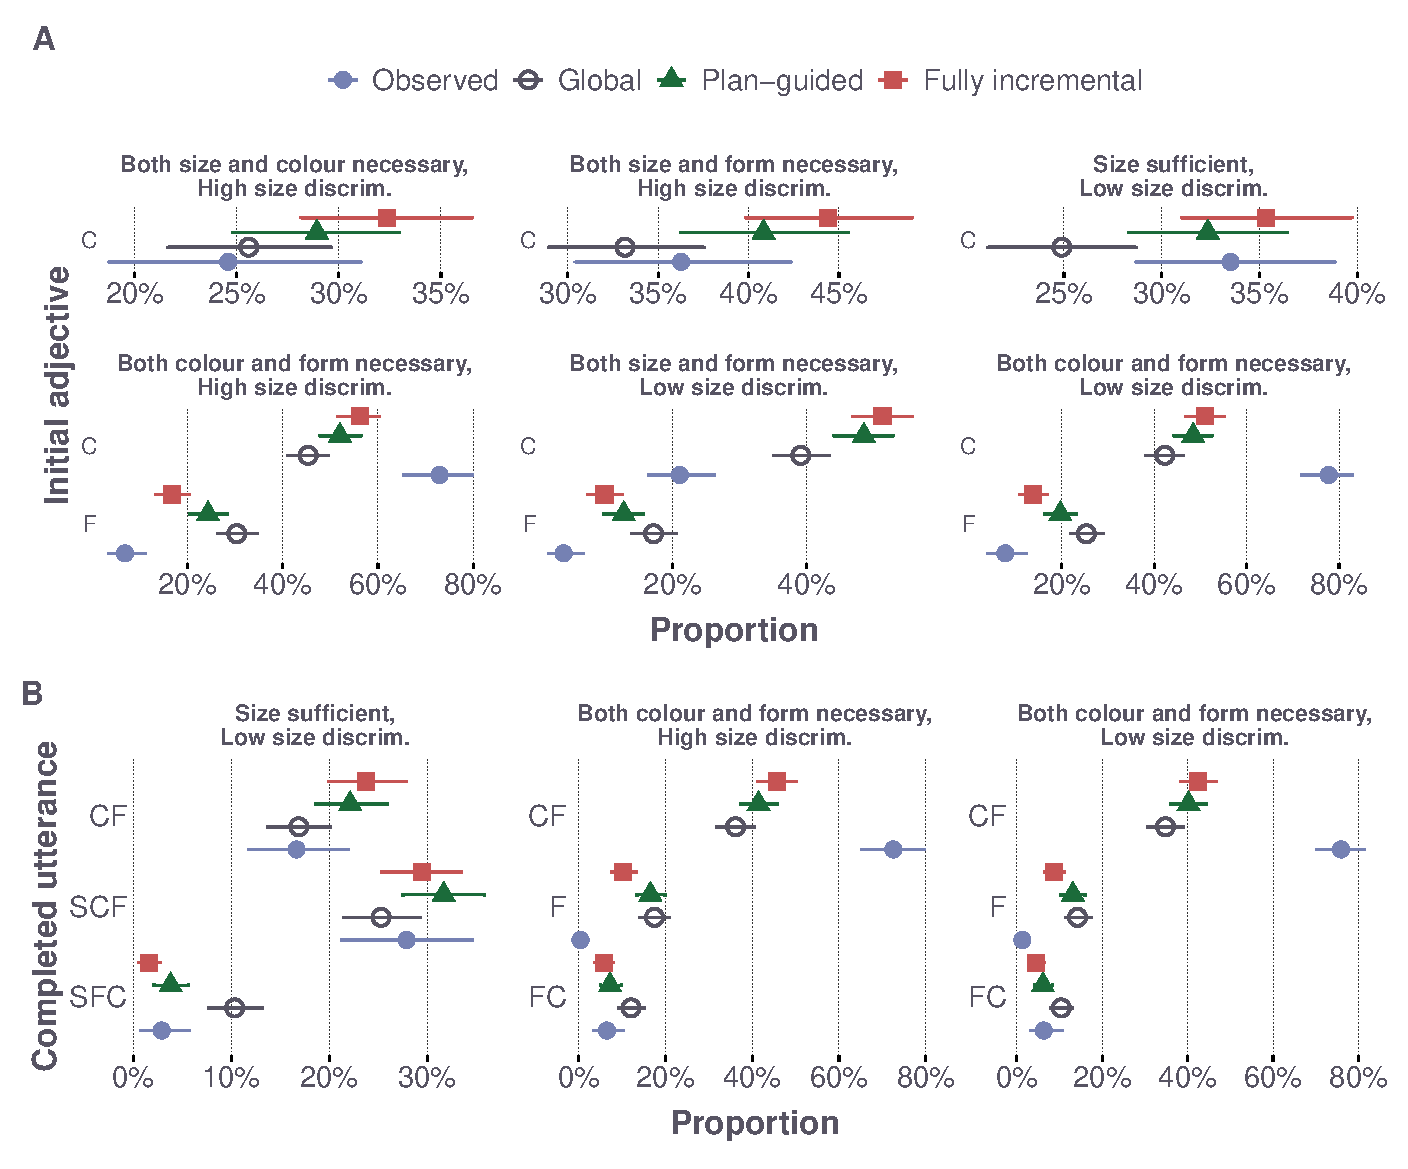
\includegraphics[width=0.95\textwidth]{production_architecture_residuals.pdf}
  \caption{Qualitative comparison of the matched production architectures.
  Panel A shows initial-adjective cells for which the maximum difference among model predictions is at least 6.7 percentage points.
  Panel B shows completed utterances with differences of at least five percentage points within the three experimental conditions with the largest pairwise total-variation distance among model predictions.
  Response labels use S for size, C for colour, and F for form.
  Intervals show participant-bootstrap 95\% intervals for observed proportions and 95\% posterior-predictive intervals for model predictions.
  Horizontal scales vary across conditions to make the comparatively small differences among production architectures visible.
  The displayed cells are descriptive diagnostics; the held-out comparison in \Cref{fig:production-architecture-results} provides the evidence for relative predictive accuracy.}
  \label{fig:production-architecture-residuals}
\end{figure}

\paragraph{Participant variation.}
The gain from participant-specific successive-choice weights also has a clear distributional location.
Participants whose posterior mean $\kappa_i$ lay farther from the shared $\kappa=.448$ gained more participant-level ELPD from the hierarchy.
The observed correlation was $r=.606$, and the participant-level Bayesian-bootstrap mean was $.627$, with a 95\% credible interval of $[.512,.756]$ and posterior probability above zero greater than $.999$.
At the response level, the hierarchy gained $214.577$ ELPD on two-adjective utterances, 95\% credible interval $[151.759,302.283]$, and $177.423$ ELPD on three-adjective utterances, 95\% credible interval $[97.047,295.251]$.
Its contribution to one-adjective utterances was $-39.849$ ELPD, with a 95\% credible interval of $[-64.418,-16.247]$.
The participant hierarchy therefore improves prediction where speakers traverse multi-adjective paths and successive alternatives can redistribute probability among completed utterances.

\begin{figure}[H]
  \centering
  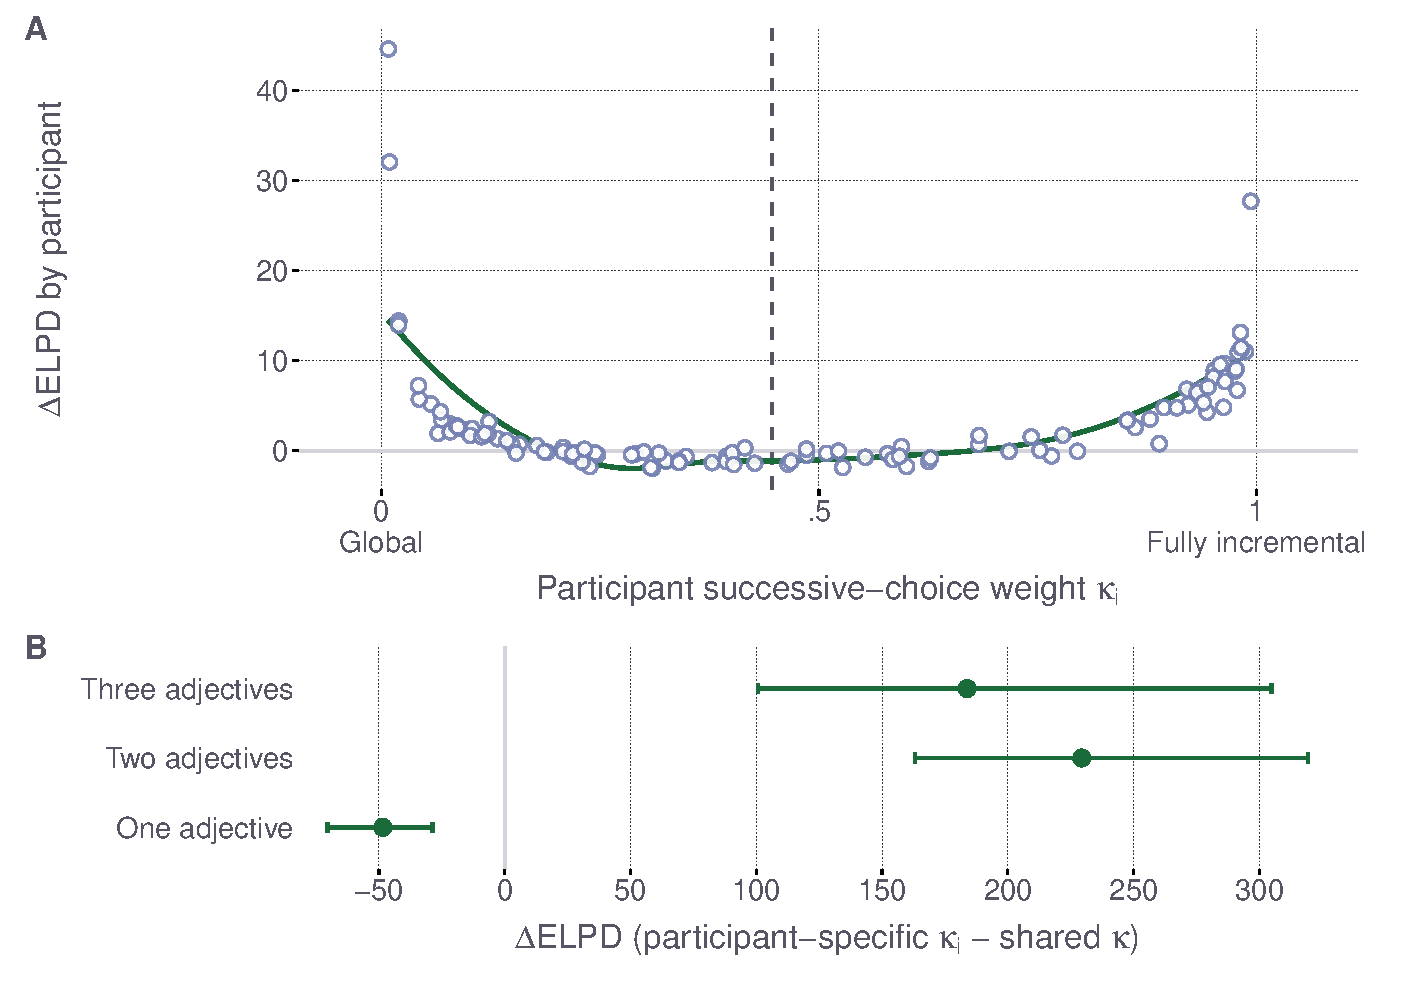
\includegraphics[width=0.95\textwidth]{production_kappa_hierarchy_diagnostics.pdf}
  \caption{Where participant-specific successive-choice weights improve prediction.
  Panel A relates each participant's leave-one-out gain from the $\kappa_i$ hierarchy to their posterior mean $\kappa_i$; the dashed line marks the shared-$\kappa$ estimate and the curve is a descriptive smooth.
  Panel B decomposes the total ELPD gain by observed response length.
  Intervals in Panel B are 95\% credible intervals from the participant-level Bayesian bootstrap.
  Both panels use the best-fitted plan-guided model and its otherwise matched shared-$\kappa$ ablation to localise the held-out model contrast.}
  \label{fig:production-kappa-hierarchy}
\end{figure}

The joint participant hierarchy includes variation in pragmatic optimality $\alpha_i$ and stable-order weight $\beta_i$ alongside variation in $\kappa_i$.
Posterior-predictive contrasts between participants in the lower and upper tails of each parameter localise their fitted response signatures.
Higher $\alpha_i$ concentrates probability on a sufficient single adjective, especially S in size-sufficient displays and F in form-sufficient displays.
Higher $\kappa_i$ mainly redistributes probability among form-involving responses whose continuation sets differ after the first adjective.
Higher $\beta_i$ shifts probability from single-adjective responses towards longer responses that follow the stable order score.
The posterior participant-level association between $\kappa_i$ and $\beta_i$ was positive and moderate, with mean $r=.291$ and 95\% credible interval $[.200,.376]$.
The associations of $\alpha_i$ with $\kappa_i$ and $\beta_i$ were centred near zero.
These tail contrasts are derived from the same joint fit and clarify the distributional interpretation of the parameters; independent observations across tasks or sessions would be required to identify corresponding participant strategies.

Maximal three-adjective utterances accounted for 1{,}633 of the 9{,}100 modelled responses, or 17.9\%.
Within the fitted model, these responses balance accumulated referential value and salience against a shared three-adjective cost, with $\alpha_i$, $\kappa_i$, and $\beta_i$ determining how that balance is expressed for each participant.
The predictive gain on three-adjective utterances shows that participant variation in successive adjective choice helps locate these responses in the observed distribution.
\FloatBarrier

\paragraph{Claim scope.}
\label{sec:production-scope}
The architecture and hierarchy contrasts assess prediction of completed utterances.
The localisation plots use the same fitted data, and their evidential role is to locate the already established held-out gains within the response distribution.
A reduced task link preserved the relative predictive advantage of plan-guided production and substantially reduced absolute predictive accuracy.
The production account therefore requires both a model of how utterances are evaluated and a task link for adjective selection and length.
The full model-development and participant-identification analyses appear in \Cref{sec:appendix:auxiliary-models,sec:appendix:participant-audit}.
Individual online planning profiles remain outside the evidence supplied by these data.
\FloatBarrier


% =============================================================================
\section{Sequential Context Updating within Hierarchical Semantic Composition}
\label{sec:simulation}
% =============================================================================

\subsection{Conditions for an Order Asymmetry}
\label{sec:simulation:boundary}

The simulation removes the fitted stable-order component, visual-salience calibration, task link, and participant variation.
Both surface orders are interpreted by a hierarchically compositional listener that combines the noun-adjacent adjective first.
The simulation crosses global and fully incremental production with context-fixed semantics and sequential context updating over a broad grid of context sizes, size distributions, colour reliability, threshold selectivity, and perceptual blur.
Full grid details appear in \Cref{sec:appendix:sim-params}.

For each simulated context, the analysis computes the pragmatic listener's target probability after \emph{big blue} and after \emph{blue big}.
The size-first advantage is
\begin{equation}
  \Delta_{\mathrm{SF}}
  =L_1(o^*\mid\text{``big blue''})
  -L_1(o^*\mid\text{``blue big''}).
  \label{eq:simulation-advantage}
\end{equation}
Positive values indicate a higher model-assigned target probability for the size-first order.

\begin{figure}[H]
  \centering
  
\includegraphics[width=0.90\textwidth]{sim_advantage_nobj.pdf}
  \caption{Boundary simulation of the size-first advantage $\Delta_{\mathrm{SF}}$ as a function of context size and contextual spread, faceted by production account and semantic regime. Positive values indicate a higher model-assigned target probability for the size-first order. The figure characterises model behaviour under simulated assumptions and leaves participants' use of the mechanism open.}
  \label{fig:sim-nobj}
\end{figure}

Sequential context updating produces a positive size-first advantage across much of the high-reliability simulation grid, including under global production.
The global context-fixed model assigns the same target probability to the two orders.
Fully incremental production changes the shape of the asymmetry and can yield a colour-first advantage when size is weak and the context is small.
The simulation identifies generative sufficiency and its boundary conditions.
Its evidential target is the behaviour generated by the model under controlled assumptions.


% =============================================================================
\section{General Discussion}
\label{sec:discussion}
% =============================================================================

The behavioural studies place adjective ordering within the broader problem of reference generation.
Explicit slider judgements exhibit a replicated context gradient: size-first preference is strongest when size identifies the target, weakest when colour does, and remains slightly positive in colour-sufficient scenes.
Production distributes the same contextual pressure across a larger response space.
Speakers often select one sufficient adjective, and visual size reliability primarily affects whether they add material.
On those trials, selection and utterance length determine whether a multi-adjective ordering decision arises at all.

The final production comparison evaluates that complete response space.
With participant-specific variation in pragmatic optimality and stable order expectations controlled, plan-guided incremental production outpredicts both global and fully incremental production.
The population location of the successive-choice weights lies between these endpoints, and participants vary widely around it.
The matched architecture advantage is concentrated in colour-initial responses, and the participant hierarchy gains predictive accuracy primarily on multi-adjective utterances.
The central computational result concerns the probability distribution over completed utterances and leaves the temporal implementation of planning open.

Stable order expectations enter through a German language-model residual whose influence varies across participants.
The model treats this conventional size-first tendency as a controlled source of variation.
Accurate prediction of adjective selection and length additionally requires a task link for salience, adjective sufficiency, form use, visual reliability, and utterance length.
A reduced task link preserves the relative advantage of plan-guided production and incurs a substantial loss in absolute predictive accuracy.
Plan-guided production operates within a broader account of the task decisions that make an adjective order observable.

The two directional accounts of communicative efficiency receive different forms of evidence.
The predictive contribution of sequential context updating within hierarchical semantic composition is practically negligible in the present materials.
Controlled simulation shows that the same operation can create a size-first target-probability advantage when colour is more reliable and the semantic update is less diffuse.
That result establishes a possible semantic route under the implemented assumptions.
The fitted predictive gain lies in production architecture, and the simulation establishes generative sufficiency for hierarchical semantic composition.
Participants' use of the simulated semantic route remains open.

\subsection{Participant Variation and Redundant Production}

The participant hierarchy locates individual variation along pragmatic optimality, successive adjective choice, and stable order expectations.
The cognitive sources of these distributional dimensions remain underdetermined, especially for maximal three-adjective descriptions.
Egocentric accounts predict redundant production when perceptually accessible properties are encoded early and omitting them would require additional planning \citep{pechmann1989incremental,engelhardt2006speakers}.
Audience-oriented accounts predict redundant production when additional properties can guide visual search or hedge uncertainty about the cues available to the listener \citep{rubio2016redundant,rubio2019overinformative,degen2020redundancy,tourtouri2021rational}.
Both pressures can converge on the same completed utterance in a shared visual task.
Independent manipulations of property accessibility, partner knowledge, and listener uncertainty would be required to distinguish their contributions.
The participant parameters and response signatures in Section~5 provide distributional targets for these tests.

\subsection{Resource Bounds and Competing Efficiency Pressures}

The production model exposes a computational limit of closed-world RSA models, for which scalability and cognitive boundedness remain general challenges \citep{degen2023rational}.
With $d$ available adjectives and no repetition, the number of ordered non-empty strings is $|\mathcal U_d|=\sum_{k=1}^{d}d!/(d-k)!$: the present three-adjective vocabulary yields 15 responses, four adjectives yield 64, five yield 325, and ten yield almost ten million.
Each response must additionally be evaluated across its surface prefixes and possible referents, and sequential context updating can require the interpretation of size to be recomputed after a semantic restriction.
The present model uses one pragmatic speaker level; its computational burden arises from this exact enumeration, repeated semantic composition, and local normalisation within every Bayesian likelihood evaluation.

Precomputed response and prefix structures, vectorised and compiled JAX operations, GPU execution, and NumPyro inference make exact fitting feasible for the present fifteen-response space.
The same implementation leaves open how a speaker model should operate when the adjective vocabulary, referential context, and set of possible utterances are substantially larger.
This boundary matters for cognitive interpretation because computational-level theories are constrained by the resources available to the system that implements them \citep{vanrooij2008tractable}.

A resource-bounded extension could retrieve or sample a limited set of salient utterances, use a top-$k$ or beam approximation to continuation sets, or estimate prefix normalisers through importance sampling.
These approximations would need to be evaluated against the exact model under controlled computational budgets, using held-out predictive accuracy and the qualitative production-architecture diagnostics as joint criteria.
Approximation can introduce systematic inferential errors, so preservation of the present fit and parameter interpretation would remain an empirical result \citep{kwisthout2011bayesian}.
This comparison would connect plan-guided production to resource-rational analysis by asking which approximate computations achieve the highest communicative value for their computational cost \citep{lieder2020resource}.

The competing pressures in the model define a related multi-objective problem.
Referential success, early informativeness, stable order expectations, utterance length, and computational effort can favour different responses.
Losses on one objective that accompany gains on another define a \emph{Pareto trade-off}; a weighted RSA utility selects one compromise among these objectives.
Related information-theoretic work characterises pragmatic reasoning as a trade-off between expected utility and communicative effort \citep{zaslavsky2021rate}.
The present comparison shows that plan-guided production predicts the observed compromise better than its endpoints.
Pareto optimality remains untested in the present analyses.
A resource-bounded comparison could trace a predictive-accuracy--computation frontier and ask whether similar fit can be retained with fewer utterance alternatives or fewer local normalisations.

\subsection{Process and Generalisation}

Hierarchical composition specifies which semantic restriction is computed inside another in a formal representation.
Plan-guided production specifies how an advance utterance plan and successive surface choices jointly shape completed utterance probabilities.
The millisecond time course of semantic interpretation and utterance planning remains open for both operations.
Online measures would be needed to identify temporal implementation.

The experiments use German prenominal noun phrases in a controlled reference task with a fixed adjective vocabulary and a restricted fifteen-response support.
The treatment of form supports prediction, and the stable order component is imported from a language model.
Further work can test whether the architecture generalises to freer production, new lexical families, different adjective systems, and designs that independently manipulate lexical subjectivity and perceptual reliability.
Such extensions should preserve the distinction between response-space prediction, semantic sufficiency, and process identification.

Taken together, the results locate adjective order within choices about what to mention and how much to say.
Within that response-generation problem, completed utterances are predicted best by plan-guided incremental production, in which an advance utterance plan constrains production while successive adjective choices continue to shape the final response.


\section{Data Availability Statement}

Data, analysis scripts, model code, final posterior summaries, and figure-generation scripts will be made available in an anonymised repository upon submission.
The repository will include the deterministic production input, the final global, plan-guided, and fully incremental model artifacts, preprocessing and reconstruction receipts, and the scripts required to reproduce the reported behavioural and predictive analyses.

\section{Author Note}

Acknowledgements, funding information, author contributions, and competing-interest statements will be finalised with the author team before journal submission.

% =============================================================================
\printbibliography
% =============================================================================
\appendix

\section{Methods and Coding Transparency}
\label{sec:appendix:methods-transparency}

\Cref{tab:exclusion-transparency} summarises the participant exclusions and the analysis tables used in the reported manuscript analyses.
The per-criterion exclusion counts are not mutually exclusive, so the unique number of excluded participants is smaller than the sum of the criterion counts.
For Study~2, the canonical production table contains all three adjective-pair families.
The production model comparison reported in \Cref{sec:modelcomparison} uses all 9{,}100 canonical annotated observations over the 15 utterance categories and three adjective-family pairings.
The size--colour marginal is retained as the theoretical anchor and descriptive subset.

\begin{table}[H]
\centering
\caption{Participant exclusions and analysis-table sizes.
Criterion counts overlap within study.}
\label{tab:exclusion-transparency}
\footnotesize
\setlength{\tabcolsep}{3pt}
\renewcommand{\arraystretch}{0.96}
\begin{tabularx}{\textwidth}{>{\raggedright\arraybackslash}p{2.0cm}>{\raggedright\arraybackslash}p{2.5cm}>{\raggedright\arraybackslash}p{5.7cm}>{\raggedright\arraybackslash}X}
\hline
Experiment & Starting and final $N$ & Participant exclusions & Analysis table used in manuscript \\
\hline
Study 1a slider ratings & $150 \rightarrow 134$ & $8$ with more than three missing trial-list entries; $8$ with extreme completion time; $2$ with more than three control-item failures; $6$ with more than three ``none fits'' responses on experimental items; $16$ unique participants excluded.
& Broad cleaned critical table: $10{,}606$ observations.
Reported size--colour slider subset: $3{,}485$ observations. \\
Study 1b slider replication & $132 \rightarrow 104$ & $6$ missing-list failures; $1$ duration failure; $3$ control failures; $24$ experimental none-fit failures; $28$ unique participants excluded.
& Cleaned replication table: $8{,}379$ critical observations.
Reported size--colour slider subset: $2{,}786$ observations. \\
Production study & $149 \rightarrow 113$ & $8$ with extreme completion time; $25$ with more than $80\%$ identical responses; $7$ with more than $10\%$ missing or unannotatable responses; $36$ unique participants excluded.
& Canonical full-data table: $9{,}100$ annotated observations.
Reported size--colour behavioural subset: $3{,}034$ observations. \\
\hline
\end{tabularx}
\end{table}

The slider-rating materials used the fixed adjective vocabulary in \Cref{tab:slider-vocabulary}.
The raw stimulus table encodes colours and forms with compact feature labels; the interface displayed the corresponding German adjective forms in phrases such as \emph{den gro{\ss}en blauen Aufkleber}.

\begin{table}[H]
\centering
\caption{Adjective vocabulary in the slider-rating item descriptions.}
\label{tab:slider-vocabulary}
\footnotesize
\begin{tabularx}{\textwidth}{p{2.2cm}p{4.5cm}X}
\hline
Property class & Raw stimulus values & German adjective forms displayed in the item text \\
\hline
Size & Numeric size levels \texttt{1--6}, \texttt{9}, \texttt{10} & \emph{gro{\ss}en}, \emph{kleinen} \\
Colour & \texttt{blue}, \texttt{orange}, \texttt{grey}, \texttt{brown}, \texttt{green}, \texttt{black} & \emph{blauen}, \emph{orangen}, \emph{grauen}, \emph{braunen}, \emph{gr\"unen}, \emph{schwarzen} \\
Form & \texttt{circle}, \texttt{diamond}, \texttt{heart}, \texttt{quadrat}, \texttt{star}, \texttt{triangle} & \emph{runden}, \emph{diamantf\"ormigen}, \emph{herzf\"ormigen}, \emph{quadratischen}, \emph{sternf\"ormigen}, \emph{dreieckigen} \\
\hline
\end{tabularx}
\end{table}

The final modelling table is reconstructed deterministically from the raw stimulus records.
Observed colour and form values are recoded into target--object relations without stochastic nuisance-feature generation; this recoding is separate from the lexical forms shown to participants.

Production responses were coded into the 15 ordered adjective categories listed in \Cref{tab:production-coding}.
The data files use \texttt{D} for the size or dimension adjective.
The model exposition uses \adj{S}; the two notations refer to the same adjective class.
Misspellings and transparent lexical alternatives were normalised when their semantic class was unambiguous.
Spatial descriptions, comparative or ordinal size expressions, and responses that could not be assigned to a target adjective class were excluded from the production model comparison.

\begin{table}[H]
\centering
\caption{Production coding dictionary.
In the data files, \texttt{D} corresponds to the size adjective \adj{S}; \texttt{C} and \texttt{F} correspond to colour and form.}
\label{tab:production-coding}
\footnotesize
\begin{tabularx}{0.85\textwidth}{p{2.4cm}X}
\hline
Length & Codes \\
\hline
One adjective & \texttt{D}, \texttt{C}, \texttt{F} \\
Two adjectives & \texttt{DC}, \texttt{DF}, \texttt{CD}, \texttt{CF}, \texttt{FD}, \texttt{FC} \\
Three adjectives & \texttt{DCF}, \texttt{DFC}, \texttt{CDF}, \texttt{CFD}, \texttt{FDC}, \texttt{FCD} \\
\hline
\end{tabularx}
\end{table}

The behavioural hypotheses were evaluated with Bayesian hierarchical models.
All analyses used the size--colour subsets reported in the main experiment figures: 3{,}485 observations in Study~1a, 2{,}786 in Study~1b, and 3{,}034 in Study~2.
The later production-model comparison addresses predictive differences among the proposed computational mechanisms over the complete fifteen-category response space and all 9{,}100 production trials.
For the slider analyses, ratings were reoriented toward size-first, divided by 100, and centred by subtracting $0.5$.
Let $\mathbf{x}_{ij}$ encode referential context, size discriminability, and their interaction, and let $\mathbf{z}_{ij}$ encode the participant intercept and context slopes.
The slider models used a Gaussian likelihood with
\[
  y_{ij}\sim\operatorname{Normal}(\mu_{ij},\sigma),
  \qquad
  \mu_{ij}=\mathbf{x}_{ij}^{\mathsf T}\boldsymbol\beta+\mathbf{z}_{ij}^{\mathsf T}\mathbf{b}_{i},
  \qquad
  \mathbf{b}_{i}\sim\operatorname{MVN}(\mathbf{0},\boldsymbol\Sigma_{\mathrm{participant}}).
\]
For production, size-initiality indicated whether the coded response began with the size adjective.
Over-informativeness indicated a three-adjective response in both-necessary contexts or a multi-adjective response in one-property-sufficient contexts.
Both binary outcomes used a Bernoulli likelihood with a logit link and an item intercept $c_k$:
\[
  y_{ijk}\sim\operatorname{Bernoulli}(\pi_{ijk}),
  \qquad
  \operatorname{logit}(\pi_{ijk})=\mathbf{x}_{ijk}^{\mathsf T}\boldsymbol\beta+\mathbf{z}_{ijk}^{\mathsf T}\mathbf{b}_{i}+c_k,
  \qquad
  c_k\sim\operatorname{Normal}(0,\sigma_{\mathrm{item}}).
\]
For the slider studies, the interaction was represented by two posterior contrasts: the high-minus-low discriminability effect in the both-necessary context minus the corresponding effect in the size-sufficient context, and the high-minus-low effect in the colour-sufficient context minus the effect in the size-sufficient context.
The production interactions were planned contrasts on the posterior-predictive probability scale.
For size-initiality, the contrast was the high-minus-low discriminability effect in the both-necessary context minus the mean effect in the two one-property-sufficient contexts.
For over-informativeness, the contrast was the low-minus-high discriminability effect in the size-sufficient context minus the mean effect in the both-necessary and colour-sufficient contexts.

The slider models used a Gaussian likelihood, correlated participant intercepts and context slopes, $\operatorname{Normal}(0,.30)$ priors on fixed effects, $\operatorname{HalfNormal}(.20)$ priors on participant standard deviations, and a $\operatorname{HalfNormal}(.25)$ prior on residual standard deviation.
The production models used Bernoulli likelihoods, the same correlated participant effects, an item intercept, a $\operatorname{Normal}(0,2)$ intercept prior, $\operatorname{Normal}(0,1.5)$ priors on the remaining fixed effects, and $\operatorname{HalfNormal}(1)$ priors on participant and item standard deviations.
Participant-effect correlations received an LKJ$(2)$ prior.
Four vectorized chains each provided $1{,}000$ retained draws after $1{,}000$ warm-up iterations.
All four fits had zero divergences, no maximum-tree-depth hits, $\widehat{R}\leq1.01$, and minimum effective sample sizes above $900$.
For each posterior draw, posterior-predictive cell expectations were computed for a new participant and, in production, a new item by integrating over the fitted random-effects distributions.
The planned predictive hypotheses were then evaluated on the rating or response-probability scale.
The analysis records cell predictions, planned hypothesis contrasts, and inference diagnostics for all four fits.



\section{Final Production Model Specification}
\label{sec:appendix:model-specification}
\label{sec:appendix:inventory}

\subsection{Deterministic Input Reconstruction}

The final production input is reconstructed one-to-one from the raw stimulus table using participant list, condition, and item identifiers.
Each retained response is paired with one observed $6\times3$ display tensor containing size, colour, and form values.
An earlier preprocessing pipeline generated nuisance-feature values stochastically for some nominally irrelevant dimensions; the final analysis removes this transformation.
Legacy first-draw, last-draw, and agreement-subset analyses are retained only as reproducibility sensitivities.
The architecture and semantic-boundary conclusions are qualitatively stable across those legacy specifications.

\subsection{Graded Size Meaning}

Size is represented by a graded threshold over the scene-level comparison class $\mathcal C$ \citep{schmidt2009how,franke2019subjectivity}:
\begin{equation}
  \theta_{\delta}(\mathcal C)
  = Q_{.80}(\mathcal C)
    - \delta\,\bigl(Q_{.80}(\mathcal C)-Q_{.20}(\mathcal C)\bigr),
  \label{eq:size-threshold}
\end{equation}
where $Q_{.20}$ and $Q_{.80}$ are probability-weighted size quantiles and $\delta$ controls threshold selectivity.
The implementation applies a perceptual-blur function around this threshold, yielding graded size-membership values.
\Cref{eq:prefix-listener,eq:prefix-raw-utility,eq:path-components,eq:plan-guided-speaker} define how this meaning enters the literal listener and the three production accounts.

\subsection{Component Inventory}

\begin{table}[H]
\centering
\caption{Final production-model components.}
\label{tab:final-component-inventory}
\footnotesize
\begin{tabularx}{\textwidth}{p{2.6cm}p{2.0cm}X}
\toprule
Component & Status & Role \\
\midrule
Observed display input & Fixed & All visible size, colour, and form values \\
Size threshold and blur & Fixed constants & Graded size meaning in the scene comparison class \\
Colour reliability & Fixed & Soft determinate colour meaning \\
Form reliability & Fixed neutral & Form production supported by the task link \\
Pragmatic rationality & Estimated, hierarchical & Participant variation in response concentration \\
Stable-order score $\Omega$ & Fixed feature & Relative order expectation within adjective sets \\
Stable-order weight $\beta_i$ & Estimated, hierarchical & Participant variation in stable order expectation \\
Salience coefficient & Estimated & Display prominence in candidate utility \\
Task-link coefficients & Estimated & One-word support, form backup, length and reliability terms \\
Successive-choice weight $\kappa_i$ & Estimated, hierarchical, in plan-guided production & Participant variation in successive adjective choice \\
\bottomrule
\end{tabularx}
\end{table}

\todo{Insert the frozen prior inventory for the final plan-guided production model.}

\section{Production Account Comparison and Diagnostics}
\label{sec:appendix:model-diagnostics}

\begin{table}[H]
\centering
\caption{Bayesian-bootstrap contrasts for the matched production architectures and the plan-guided participant hierarchy.}
\label{tab:final-architecture-contrasts}
\footnotesize
\begin{tabularx}{\textwidth}{Xrrr}
\toprule
Contrast & $\Delta$ELPD & 95\% credible interval & $P(\Delta>0)$ \\
\midrule
Plan-guided, shared $\kappa$, minus average endpoints & $326.280$ & $[241.632,417.363]$ & $>.999$ \\
Fully incremental minus global & $-192.079$ & $[-573.371,84.802]$ & $.106$ \\
Participant $\kappa_i$ hierarchy, context-fixed & $351.425$ & $[239.353,503.120]$ & $>.999$ \\
Participant $\kappa_i$ hierarchy, updating & $352.150$ & $[240.022,504.081]$ & $>.999$ \\
\bottomrule
\end{tabularx}
\end{table}

All six models in the matched factorial comparison used four chains, 1{,}000 warm-up iterations, and 1{,}000 retained draws.
They had zero divergences, maximum $\widehat R<1.007$, minimum BFMI above $.640$, and no observation with Pareto $k>.7$.
In both semantic regimes, the exact endpoint audit returned maximum probability and log-probability differences of zero when the shared successive-choice weight in plan-guided production was fixed at $\kappa=0$ or $\kappa=1$.

\section{Model-Development Checks}
\label{sec:appendix:auxiliary-models}

\paragraph{Form package.}
The selected form specification fixes form reliability at $.50$ and estimates a form-use coefficient in the task link.
Two fixed informative alternatives tied form reliability to the colour value, with either the original or a strongly shrunk backup prior.
The alternatives had lower predictive accuracy in the full response space.
This comparison supports the selected form specification as an auxiliary predictive component and leaves participants' lexical semantics for form open.

\paragraph{Stable order source.}
The selected specification uses the German language-model residual alone.
Adding a reliability-order term yielded worse conditional-order prediction within fixed adjective sets.
Models that removed the language-model residual yielded invalid posterior or PSIS evidence.
The comparison rejects the proposed reliability addition and leaves the cognitive source of stable order expectations open.

\paragraph{Task link.}
The reduced task-link comparison removed the sufficient-one-word bonus, form-use term, three-word penalty, and size-reliability terms as one bundle.
Plan-guided production retained its relative advantage over both endpoints, while all reduced models lost substantial absolute predictive accuracy.

\todo{Insert the compact numerical tables for the auxiliary form, stable-order, and reduced task-link comparisons.}

\section{Participant Hierarchy Audit}
\label{sec:appendix:participant-audit}

The participant hierarchy audit first fitted separate extensions of the shared-$\kappa$ model.
That screen showed that participant-specific successive-choice and stable-order variation could absorb similar predictive structure when fitted separately.
The final joint model estimates pragmatic optimality, successive-choice weight, and stable-order weight simultaneously.
Relative to the otherwise matched shared-$\kappa$ model, the joint hierarchy gained $351.425$ ELPD under context-fixed semantics, 95\% credible interval $[239.353,503.120]$, and $352.150$ ELPD under sequential context updating, 95\% credible interval $[240.022,504.081]$.
Its sampler and PSIS diagnostics passed the registered thresholds.
The participant-level posterior correlations were $.001$ for $\alpha_i$ with $\kappa_i$, $-.080$ for $\alpha_i$ with $\beta_i$, and $.291$ for $\kappa_i$ with $\beta_i$.
Descriptive correlations and tail-group predictions decode the latent parameters within the fitted model and provide no independent validation.

\section{Endpoint Identity and Architecture Audit}
\label{sec:appendix:normalisation-audit}

At common parameter values, plan-guided production with $\kappa=0$ exactly recovers global production, and with $\kappa=1$ exactly recovers fully incremental production.
The participant-specific order mapping, terminal response-policy kernel, and response support are identical across the three architectures.
Maximum category-probability and log-probability differences were zero at a numerical tolerance of $10^{-10}$.

\section{Sequential Context Updating for Size}
\label{sec:appendix:semantic-details}

For the hierarchical semantic path, let $H_{j-1}$ be the state after the syntactically inner modifiers have composed.
The context-updating listener recomputes the size threshold from this hierarchically prior state:
\begin{equation}
  \llbracket \adj{S}\rrbracket_{\mathrm{upd},H_{j-1}}(o)
  =\llbracket \adj{S}\rrbracket_{\theta_{\delta}(H_{j-1})}(o),
  \label{eq:context-updating}
\end{equation}
The context-fixed listener anchors the threshold to the scene prior:
\begin{equation}
  \llbracket \adj{S}\rrbracket_{\mathrm{fix}}(o)
  =\llbracket \adj{S}\rrbracket_{\theta_{\delta}(P_0)}(o).
  \label{eq:context-fixed}
\end{equation}
For \emph{big blue}, hierarchical composition applies the colour restriction before interpreting size.
The distinct surface production calculation follows left-to-right order and uses the validated factorisation in which every meaning is applied once.
The matched observed-display comparison yielded no practically meaningful predictive difference between fixed and sequentially updated comparison classes.

\section{Simulation Parameter Sweeps}
\label{sec:appendix:sim-params}

\Cref{fig:sim-k,fig:sim-wf,fig:sim-csv} show how the three fixed semantic parameters affect communicative success across the two speaker architectures.

\begin{table}[H]
  \caption{Simulation parameter grid}
  \label{tab:simulation}
  \centering
  \begin{tabularx}{0.92\textwidth}{lXl}
    \toprule
    \textbf{Parameter} & \textbf{Grid values} & \textbf{\# levels} \\
    \midrule
    Speaker architecture & Incremental, global & 2 \\
    Semantic regime & Context-updating, context-fixed & 2 \\
    $n_\text{obj}$ & 2, 6, 10, 14, 18, 22, 26, 30 & 8 \\
    $\sigma_\text{spread}$ & 2.0, 7.75, 15.0 & 3 \\
    $\nu$ & 0.90, 0.92, 0.94, 0.96, 0.98 & 5 \\
    $k$ & 0.10, 0.30, 0.50, 0.70, 0.90 & 5 \\
    $w_f$ & 0.1, 0.2, 0.3, 0.5, 0.8 & 5 \\
    \midrule
    Random context samples per combination & 1{,}000 & \\
    \midrule
    \textbf{Total trials} & \textbf{12{,}000{,}000} & \\
    \bottomrule
  \end{tabularx}
\end{table}

\begin{figure}[H]
  \centering
  
\includegraphics[width=0.86\textwidth]{sim_k.pdf}
  \caption{Effect of the threshold parameter $k$ on communicative success in the simulation.}
  \label{fig:sim-k}
\end{figure}

\begin{figure}[H]
  \centering
  
\includegraphics[width=0.86\textwidth]{sim_wf.pdf}
  \caption{Effect of perceptual blur $w_f$ on communicative success in the simulation.}
  \label{fig:sim-wf}
\end{figure}

\begin{figure}[H]
  \centering
  
\includegraphics[width=0.86\textwidth]{sim_colorsemval.pdf}
  \caption{Effect of the colour semantic value $\nu$ on communicative success in the simulation.}
  \label{fig:sim-csv}
\end{figure}

% =============================================================================

\section{Slider Colour-Reliability Audit}
\label{sec:appendix:slider-nu}

The slider-rating model fixes colour reliability $\nu$ at $0.80$ in its diagnostic specification.
Production uses the softer colour value $\nu_\text{colour}=0.59$ in the production speaker (\Cref{sec:model:extended}); for parity, we apply the same kind of sensitivity audit to the slider's incremental speakers.
The audit samples $\nu \sim \mathrm{Uniform}(0.5, 0.999)$ within the model and recomputes the literal listeners at each MCMC step.
Every other component of the incremental speaker remains unchanged.
\Cref{tab:slider-nu-audit} reports the resulting posteriors alongside the originally fixed-$\nu$ fits.

\begin{table}[H]
\centering
\caption{Slider colour-reliability audit.
Fixed-$\nu$ rows use $\nu = 0.80$; free-$\nu$ rows sample $\nu \sim \mathrm{Uniform}(0.5, 0.999)$ and recompute literal listeners each step.
``ELPD'' is PSIS-LOO; ELPD loss and dse are relative to the incremental, context-updating fixed-$\nu$ model.
All four models use $4$ chains $\times$ $500$ warmup $\times$ $500$ samples; maximum split-$\hat R$ rounds to $1.01$ for the free-$\nu$ models.}
\label{tab:slider-nu-audit}
\footnotesize
\setlength{\tabcolsep}{4pt}
\begin{tabular}{p{4.2cm}rrrrrl}
\hline
Model & ELPD & ELPD loss & dse & $\alpha$ (sd) & $b$ (sd) & $\nu$ (94\% HDI) \\
\hline
\textbf{Incremental, updating, fixed $\nu = 0.80$} & $\mathbf{-2{,}774.1}$ & $\mathbf{0.0}$ & --- & $\mathbf{0.69\,(0.06)}$ & $\mathbf{0.58\,(0.06)}$ & --- \\
Incremental, fixed, fixed $\nu = 0.80$ & $-2{,}774.1$ & $0.06$ & $0.18$ & $0.69\,(0.06)$ & $0.58\,(0.06)$ & --- \\
Incremental, updating, free $\nu$ & $-2{,}775.0$ & $0.89$ & $1.08$ & $1.53\,(0.61)$ & $0.41\,(0.15)$ & $0.63\;[0.50, 0.82]$ \\
Incremental, fixed, free $\nu$ & $-2{,}774.3$ & $0.23$ & $1.00$ & $1.48\,(0.55)$ & $0.42\,(0.13)$ & $0.63\;[0.51, 0.79]$ \\
\hline
\end{tabular}
\end{table}

Three points stand out.
First, $\nu$ is weakly identified in the slider data: the updating credible interval includes the fixed value $0.80$, the fixed-semantics credible interval reaches $0.79$, and both posteriors place substantial mass near the lower prior boundary at $0.5$.
The production estimate has a narrower credible interval, $0.59\;[0.56, 0.62]$.
Second, the nominal PSIS-LOO losses are all smaller than their dse ($\mathrm{loss}/\mathrm{dse} < 1$ throughout), and the shared PSIS warnings limit these values to diagnostic use.
Third, under the freed posterior the rationality parameter $\alpha$ moves to roughly $1.5$ (from $0.69$) and the bias intercept $b$ moves below $0.5$ (from $0.58$), because $\nu$ and the other parameters trade off: a softer colour predicate forces a stronger rationality term and reduces the residual size-first bias absorbed by $b$.
We therefore retain the fixed $\nu=0.80$ for the slider model in the main text and treat $\alpha$ and $b$ at that specification as the reported quantities.
The fixed-$\nu$ estimate $b=0.58$ remains conditional on this specification, and its archived credible interval includes $0.5$.
The broader conclusion is unchanged: the slider response space weakly identifies semantic scale parameters, and the fitted PSIS-LOO comparisons remain diagnostic.


\end{document}
